% 小学数学·几何角的绘制答案
% 题目3：以下面的射线为一条边，选择合适的工具按要求画出各个角
% 编译方式：xelatex angles.tex

\documentclass[12pt, a4paper]{ctexart}

\usepackage{geometry}
\geometry{
  a4paper,
  left=2.5cm,
  right=2.5cm,
  top=2.5cm,
  bottom=2.5cm
}

\usepackage{amsmath}
\usepackage{amssymb}
\usepackage{tikz}
\usetikzlibrary{angles, quotes, arrows.meta, calc, decorations.pathreplacing}

% 绘图样式设置
\tikzset{
  ray/.style={
    -{Stealth[length=6pt]},
    line width=1.2pt,
    color=cyan!70!blue
  },
  given ray/.style={
    -,
    line width=1.2pt,
    color=cyan!70!blue
  },
  angle arc/.style={
    draw=red!70!black,
    line width=0.8pt
  },
  angle label/.style={
    font=\small,
    color=red!70!black
  },
  vertex dot/.style={
    circle,
    fill=cyan!70!blue,
    inner sep=0pt,
    minimum size=5pt
  }
}

\begin{document}

\begin{center}
  {\large\bfseries 解答：以下面的射线为一条边，画出各个角}
\end{center}

\vspace{0.5cm}

\noindent
\begin{tikzpicture}[scale=1.0]

  %% ==============================
  %% 第一图：45°角（给定射线水平向右）
  %% ==============================
  \begin{scope}[xshift=0cm]
    % 顶点
    \coordinate (A) at (0,0);
    % 给定射线（水平向右）端点
    \coordinate (B) at (3,0);
    % 答案射线（与水平线成45°）端点
    \coordinate (C) at ({3*cos(45)},{3*sin(45)});

    % 绘制给定射线（有端点，无箭头表示已给定的边）
    \draw[given ray] (A) -- (B);
    % 绘制答案射线（从顶点出发，45°方向）
    \draw[ray] (A) -- (C);

    % 顶点蓝点
    \node[vertex dot] at (A) {};

    % 角弧线
    \pic[draw=red!70!black, line width=0.8pt, angle radius=0.8cm,
         angle eccentricity=1.5, "$45°$", font=\small, color=red!70!black]
        {angle = B--A--C};

    % 标题
    \node[above] at (1.5, 2.4) {$45°$};
  \end{scope}

  %% ==============================
  %% 第二图：105°角（给定射线竖直向上）
  %% ==============================
  \begin{scope}[xshift=5.5cm]
    \coordinate (A) at (0,0);
    % 给定射线（竖直向上）
    \coordinate (B) at (0,3);
    % 答案射线方向：从竖直射线（90°）顺时针105°
    % 竖直向上=90°，顺时针105° => 90° - 105° = -15° (即从x轴正方向量取-15°)
    % 等效于从x轴正方向的 90°+105° = 195°（逆时针从右水平开始）
    % 实际上：顶角在竖直射线左侧，答案射线在右侧与给定射线夹角105°
    % 给定射线90°，若顺时针转105°，答案射线在90°-105°=-15°方向（即x轴负方向偏下15°）
    % 但通常画角是在凸侧：给定射线90°，答案射线在90°+105°=195° 或 90°-105°=-15°
    % 105°钝角，答案射线应在给定垂直射线的右侧，过渡到水平以下
    % 从给定射线(90°)顺时针转105°: 90°-105° = -15° => 即 345° = 方向(-15°)
    \coordinate (C) at ({3*cos(-15)},{3*sin(-15)});

    \draw[given ray] (A) -- (B);
    \draw[ray] (A) -- (C);
    \node[vertex dot] at (A) {};

    \pic[draw=red!70!black, line width=0.8pt, angle radius=0.7cm,
         angle eccentricity=1.6, "$105°$", font=\small, color=red!70!black]
        {angle = C--A--B};

    \node[above] at (0, 3.3) {$105°$};
  \end{scope}

  %% ==============================
  %% 第三图：165°角（比平角小15°，给定射线斜向右上方约45°）
  %% ==============================
  \begin{scope}[xshift=11cm]
    \coordinate (A) at (0,0);
    % 给定射线：斜向右上方（约45°）
    \coordinate (B) at ({2.5*cos(45)},{2.5*sin(45)});
    % 答案射线：与给定射线夹角165°
    % 给定射线方向45°，答案射线方向：45° + 165° = 210° 或 45° - 165° = -120°(=240°)
    % 取 45° - 165° = -120°，即在给定射线右侧顺时针165°
    % 从图示看给定射线斜右上，165°的另一边应在给定射线的左下侧附近
    \coordinate (C) at ({2.5*cos(45+165)},{2.5*sin(45+165)});

    \draw[given ray] (A) -- (B);
    \draw[ray] (A) -- (C);
    \node[vertex dot] at (A) {};

    \pic[draw=red!70!black, line width=0.8pt, angle radius=0.65cm,
         angle eccentricity=1.7, "$165°$", font=\small, color=red!70!black]
        {angle = B--A--C};

    \node[above right] at (1.5, 1.8) {比平角小$15°$};
    \node[below right, font=\small, color=gray] at (0.2, -0.3) {($165°$)};
  \end{scope}

\end{tikzpicture}

\vspace{1cm}
\hrule
\vspace{0.3cm}

{\small\color{gray}
\textbf{作图说明：}\\
\textcircled{1} $45°$角：用量角器，以水平射线为基准，在上方量取$45°$，画出另一条射线。\\
\textcircled{2} $105°$角：用量角器，以竖直射线为基准，在右侧量取$105°$，画出另一条射线。\\
\textcircled{3} 比平角小$15°$的角：平角$= 180°$，故所求角$= 180° - 15° = 165°$；用量角器量取即可。
}


%% ==============================
%% 第(2)题：在直线上画线段CD = 2AB
%% ==============================
\newpage

\begin{center}
  {\large\bfseries 解答：在直线上画线段 $CD$，使 $CD = 2AB$}
\end{center}

\vspace{0.8cm}

% 设定 AB 长度（单位：cm，对应 TikZ 单位）
% 图中 AB 约为斜线段，A在左下，B在右上
% 用 TikZ 计算并展示作图过程

\noindent
\begin{tikzpicture}[scale=1.1, >=Stealth]

  %% ---- 已知线段 AB（展示在左上角）----
  % A、B 的位置（模拟题图：B在A的右偏上方）
  \coordinate (A) at (0, 0);
  \coordinate (B) at (2.0, 0.8);   % AB 斜段，模拟题图

  % 画线段 AB
  \draw[line width=1.3pt, cyan!70!blue] (A) -- (B);
  \node[vertex dot] at (A) {};
  \node[vertex dot] at (B) {};
  \node[below left,  font=\small] at (A) {$A$};
  \node[above right, font=\small] at (B) {$B$};
  \node[above, font=\small\itshape, gray] at (1.0, 1.0) {线段 $AB$};

  %% ---- 右边的直线（水平线）----
  \draw[line width=1.2pt] (3.5, 0) -- (13.0, 0);

  %% ---- 作图步骤：用圆规量取 AB 长度两次 ----
  % AB 的长度（TikZ 计算）
  % |AB| = sqrt(2.0^2 + 0.8^2) = sqrt(4.64) ≈ 2.154 (TikZ单位)
  % 令 d = 2.154（即 AB 长），在水平线上截取

  % 取 C 为水平线上的起点
  \coordinate (C) at (4.5, 0);
  % 第一段：C 到 M（即 CM = AB）
  \coordinate (M) at ($ (C) + (2.154, 0) $);
  % 第二段：M 到 D（即 MD = AB，共 CD = 2AB）
  \coordinate (D) at ($ (M) + (2.154, 0) $);

  % 顶点点
  \node[vertex dot] at (C) {};
  \node[vertex dot] at (M) {};
  \node[vertex dot] at (D) {};

  % 标注 C、M、D
  \node[below, font=\small] at (C) {$C$};
  \node[below, font=\small\color{gray}] at (M) {（中点）};
  \node[below, font=\small] at (D) {$D$};

  % 标注线段
  \draw[line width=1.5pt, red!70!black] (C) -- (D);
  % 第一段 CM 标注
  \draw[<->, gray, line width=0.6pt] (C) -- (M)
      node[midway, above, font=\scriptsize] {$=AB$};
  % 第二段 MD 标注  
  \draw[<->, gray, line width=0.6pt] (M) -- (D)
      node[midway, above, font=\scriptsize] {$=AB$};
  % 整体 CD 标注
  \draw[<->, red!80!black, line width=0.8pt]
      ($ (C)+(0,-0.55) $) -- ($ (D)+(0,-0.55) $)
      node[midway, below, font=\small, red!70!black] {$CD = 2AB$};

  %% ---- 圆规弧线（示意作图过程）----
  % 第一段：以 C 为圆心，AB 为半径画弧，交直线于 M
  \draw[dashed, orange!80!black, line width=0.8pt]
      (C) ++(0:2.154) arc[start angle=0, end angle=18, radius=2.154];
  \draw[dashed, orange!80!black, line width=0.8pt]
      (C) ++(0:2.154) arc[start angle=0, end angle=-15, radius=2.154];
  % 虚线连接 C 到弧（示意圆规半径）
  \draw[dotted, orange!60, line width=0.7pt] (C) -- ($ (C)+(18:2.154) $);

  % 第二段：以 M 为圆心，AB 为半径画弧，交直线于 D
  \draw[dashed, orange!80!black, line width=0.8pt]
      (M) ++(0:2.154) arc[start angle=0, end angle=18, radius=2.154];
  \draw[dashed, orange!80!black, line width=0.8pt]
      (M) ++(0:2.154) arc[start angle=0, end angle=-15, radius=2.154];
  \draw[dotted, orange!60, line width=0.7pt] (M) -- ($ (M)+(18:2.154) $);

\end{tikzpicture}

\vspace{1cm}
\hrule
\vspace{0.4cm}

{\small\color{gray}
\textbf{作图说明（直尺和圆规法）：}\\
\textcircled{1} 用圆规量取线段 $AB$ 的长度（张开圆规，使两脚分别对准 $A$、$B$）。\\
\textcircled{2} 在直线上取一点 $C$，以 $C$ 为圆心、$AB$ 为半径画弧，弧与直线的交点记为中间点。\\
\textcircled{3} 再以该中间点为圆心、$AB$ 为半径画弧，弧与直线的交点即为点 $D$。\\
\textcircled{4} 连结 $CD$，则 $CD = 2AB$。\quad（橙色虚线弧为圆规痕迹示意）
}


%% ==============================
%% 第三题：用圆规找点B，使AB = 3厘米
%% ==============================
\newpage

\begin{center}
  {\large\bfseries 解答：用圆规在直线上找点 $B$，使 $AB = 3$ 厘米}
\end{center}

\vspace{0.8cm}

\noindent
% 此图为实际尺寸示意（1 TikZ单位 = 1cm）
\begin{tikzpicture}[scale=1.0, >=Stealth]

  %% ---- 直线（与题图一致，水平蓝线）----
  \draw[line width=1.3pt, cyan!70!blue] (-5.5, 0) -- (5.5, 0);

  %% ---- 点 A（直线中央偏左）----
  \coordinate (A) at (0, 0);
  \node[vertex dot] at (A) {};
  \node[below, font=\small] at (A) {$A$};

  %% ---- 圆规弧：以 A 为圆心，半径 3cm，画弧交直线----
  % 右侧弧（过直线上方与下方）
  \draw[dashed, orange!80!black, line width=0.9pt]
      (A) ++(0:3) arc[start angle=0, end angle=22, radius=3];
  \draw[dashed, orange!80!black, line width=0.9pt]
      (A) ++(0:3) arc[start angle=0, end angle=-18, radius=3];
  % 左侧弧
  \draw[dashed, orange!80!black, line width=0.9pt]
      (A) ++(180:3) arc[start angle=180, end angle=158, radius=3];
  \draw[dashed, orange!80!black, line width=0.9pt]
      (A) ++(180:3) arc[start angle=180, end angle=202, radius=3];

  %% ---- 辅助虚线（圆规半径示意）----
  \draw[dotted, orange!60, line width=0.7pt] (A) -- ($ (A)+(20:3) $);
  \draw[dotted, orange!60, line width=0.7pt] (A) -- ($ (A)+(160:3) $);

  %% ---- 交点 B（左右各一）----
  \coordinate (Bright) at (3, 0);
  \coordinate (Bleft)  at (-3, 0);
  \node[vertex dot, fill=red!70!black] at (Bright) {};
  \node[vertex dot, fill=red!70!black] at (Bleft)  {};
  \node[below, font=\small, red!70!black] at (Bright) {$B$};
  \node[below, font=\small, red!70!black] at (Bleft)  {$B$};

  %% ---- 尺寸标注 AB = 3厘米 ----
  % 右侧 AB
  \draw[<->, red!60!black, line width=0.7pt]
      ($ (A)+(0, 0.45) $) -- ($ (Bright)+(0, 0.45) $)
      node[midway, above, font=\small, red!70!black] {$3$ 厘米};
  % 左侧 AB
  \draw[<->, red!60!black, line width=0.7pt]
      ($ (Bleft)+(0, 0.45) $) -- ($ (A)+(0, 0.45) $)
      node[midway, above, font=\small, red!70!black] {$3$ 厘米};

\end{tikzpicture}

\vspace{1cm}
\hrule
\vspace{0.4cm}

{\small\color{gray}
\textbf{作图说明（圆规法）：}\\
\textcircled{1} 张开圆规，使两脚距离等于 $3$ 厘米（对照直尺量取）。\\
\textcircled{2} 将圆规针脚固定在点 $A$，用铅笔脚在直线上画弧。\\
\textcircled{3} 弧线与直线共有\textbf{两个交点}，均可作为点 $B$，即 $AB = 3$ 厘米。\\
（图中橙色虚弧为圆规痕迹，红点为满足条件的点 $B$）
}


%% ==============================
%% 第4题：∠1 = 50°，画∠2 = 2×∠1 = 100°
%% ==============================
\newpage

\begin{center}
  {\large\bfseries 解答：$\angle 1 = 50°$，$\angle 2 = 2 \times \angle 1 = 100°$}
\end{center}

\vspace{0.6cm}

\noindent
\begin{tikzpicture}[scale=1.1, >=Stealth]

  %%============================
  %% 左图：∠1（题目给出，测量得50°）
  %%============================
  \begin{scope}[xshift=0cm]
    \coordinate (V1) at (0, 0);       % 顶点
    \coordinate (R1) at (3.2, 0);     % 水平射线端点（向右）
    \coordinate (U1) at ({3.0*cos(50)},{3.0*sin(50)}); % 斜射线端点（50°）

    % 两条射线（青色，同题图）
    \draw[given ray] (V1) -- (R1);
    \draw[given ray] (V1) -- (U1);
    \node[vertex dot] at (V1) {};

    % 角弧 + 标注
    \pic[draw=black, line width=0.8pt, angle radius=0.75cm,
         angle eccentricity=1.55, "$1$", font=\small]
        {angle = R1--V1--U1};

    % 度数标注（红色）
    \node[red!70!black, font=\small\bfseries] at (1.5, -0.5)
        {$\angle 1 = 50°$};
  \end{scope}

  %%============================
  %% 右图：∠2 = 100°（新画）
  %%============================
  \begin{scope}[xshift=7.5cm]
    \coordinate (V2) at (0, 0);
    \coordinate (R2) at (3.2, 0);
    \coordinate (U2) at ({3.0*cos(100)},{3.0*sin(100)}); % 100°方向

    % 两条射线（青色）
    \draw[given ray] (V2) -- (R2);
    \draw[ray]       (V2) -- (U2);   % 答案射线用箭头
    \node[vertex dot] at (V2) {};

    % 角弧 + 标注
    \pic[draw=black, line width=0.8pt, angle radius=0.75cm,
         angle eccentricity=1.6, "$2$", font=\small]
        {angle = R2--V2--U2};

    % 度数标注（红色）
    \node[red!70!black, font=\small\bfseries] at (1.0, -0.5)
        {$\angle 2 = 100°$};
  \end{scope}

  %% 中间等式说明
  \node[font=\normalsize] at (5.5, 1.5)
      {$\angle 2 = 2 \times 50° = 100°$};

\end{tikzpicture}

\vspace{1cm}
\hrule
\vspace{0.4cm}

{\small\color{gray}
\textbf{解题说明：}\\
\textcircled{1} 用量角器量出左图中 $\angle 1$ 的大小，得 $\angle 1 = 50°$。\\
\textcircled{2} 计算：$\angle 2 = 2 \times \angle 1 = 2 \times 50° = 100°$。\\
\textcircled{3} 在右侧以水平射线为一边，用量角器量取 $100°$，画出另一条射线，即得 $\angle 2$。
}


%% ==============================
%% 第5题：用直尺和圆规画线段CD = 3AB
%% ==============================
\newpage

\begin{center}
  {\large\bfseries 解答：用直尺和圆规画线段 $CD$，使 $CD = 3AB$}
\end{center}

\vspace{0.6cm}

\noindent
\begin{tikzpicture}[scale=1.0, >=Stealth]

  %% ---- 已知线段 AB（左上角展示）----
  % 设 AB = 2.2（TikZ单位，约2.2cm）
  \pgfmathsetmacro{\ab}{2.2}

  \coordinate (A) at (0, 2.5);
  \coordinate (B) at (\ab, 2.5);

  \draw[line width=1.3pt, cyan!70!blue] (A) -- (B);
  \node[vertex dot] at (A) {};
  \node[vertex dot] at (B) {};
  \node[below, font=\small] at (A) {$A$};
  \node[below, font=\small] at (B) {$B$};
  \node[above, font=\small\itshape, gray] at (\ab/2, 2.7) {线段 $AB$};

  %% ---- 所画线段 CD（下方，水平）----
  % C 为起点，然后每隔AB长度打一个中间点
  \coordinate (C)  at (0,    0);
  \coordinate (M1) at (\ab,  0);          % CM1 = AB
  \coordinate (M2) at ({2*\ab}, 0);       % CM2 = 2AB
  \coordinate (D)  at ({3*\ab}, 0);       % CD  = 3AB

  % 画底线（稍长于CD，模拟直尺画出的直线）
  \draw[line width=1.0pt, gray!50] (-0.4, 0) -- ({3*\ab+0.8}, 0);

  % 红色线段CD（答案）
  \draw[line width=1.8pt, red!70!black] (C) -- (D);

  % 各点
  \node[vertex dot]                       at (C)  {};
  \node[vertex dot, fill=gray!60]         at (M1) {};
  \node[vertex dot, fill=gray!60]         at (M2) {};
  \node[vertex dot, fill=red!70!black]    at (D)  {};

  % 标注字母
  \node[below, font=\small]              at (C)  {$C$};
  \node[below, font=\small, gray]        at (M1) {};   % 中间点不标字母
  \node[below, font=\small, gray]        at (M2) {};
  \node[below, font=\small, red!70!black] at (D) {$D$};

  %% ---- 分段双箭头（各段 = AB）----
  \draw[<->, gray, line width=0.6pt]
      ($ (C)+(0, 0.45) $) -- ($ (M1)+(0, 0.45) $)
      node[midway, above, font=\scriptsize] {$=AB$};
  \draw[<->, gray, line width=0.6pt]
      ($ (M1)+(0, 0.45) $) -- ($ (M2)+(0, 0.45) $)
      node[midway, above, font=\scriptsize] {$=AB$};
  \draw[<->, gray, line width=0.6pt]
      ($ (M2)+(0, 0.45) $) -- ($ (D)+(0, 0.45) $)
      node[midway, above, font=\scriptsize] {$=AB$};

  %% ---- 总长标注 CD = 3AB ----
  \draw[<->, red!80!black, line width=0.9pt]
      ($ (C)+(0,-0.6) $) -- ($ (D)+(0,-0.6) $)
      node[midway, below, font=\small, red!70!black] {$CD = 3AB$};

  %% ---- 圆规弧示意（以 C、M1、M2 为圆心，AB为半径）----
  % 弧1：以 C 为圆心
  \draw[dashed, orange!80!black, line width=0.8pt]
      (C) ++({0:\ab}) arc[start angle=0, end angle=18,  radius=\ab];
  \draw[dashed, orange!80!black, line width=0.8pt]
      (C) ++({0:\ab}) arc[start angle=0, end angle=-15, radius=\ab];
  \draw[dotted, orange!60, line width=0.6pt] (C) -- ($ (C)+(18:\ab) $);

  % 弧2：以 M1 为圆心
  \draw[dashed, orange!80!black, line width=0.8pt]
      (M1) ++({0:\ab}) arc[start angle=0, end angle=18,  radius=\ab];
  \draw[dashed, orange!80!black, line width=0.8pt]
      (M1) ++({0:\ab}) arc[start angle=0, end angle=-15, radius=\ab];
  \draw[dotted, orange!60, line width=0.6pt] (M1) -- ($ (M1)+(18:\ab) $);

  % 弧3：以 M2 为圆心
  \draw[dashed, orange!80!black, line width=0.8pt]
      (M2) ++({0:\ab}) arc[start angle=0, end angle=18,  radius=\ab];
  \draw[dashed, orange!80!black, line width=0.8pt]
      (M2) ++({0:\ab}) arc[start angle=0, end angle=-15, radius=\ab];
  \draw[dotted, orange!60, line width=0.6pt] (M2) -- ($ (M2)+(18:\ab) $);

\end{tikzpicture}

\vspace{1cm}
\hrule
\vspace{0.4cm}

{\small\color{gray}
\textbf{作图说明（直尺和圆规法）：}\\
\textcircled{1} 用圆规量取线段 $AB$ 的长度。\\
\textcircled{2} 在纸上用直尺画一条射线，取一端点为 $C$。\\
\textcircled{3} 以 $C$ 为圆心、$AB$ 为半径画弧，交射线于中间点（第1次截取）。\\
\textcircled{4} 再以该点为圆心、$AB$ 为半径画弧，交射线于第二个中间点（第2次截取）。\\
\textcircled{5} 再以第二个中间点为圆心、$AB$ 为半径画弧，交射线于点 $D$（第3次截取）。\\
\textcircled{6} 线段 $CD$ 即为所求，$CD = 3AB$。\quad（橙色虚弧为圆规痕迹示意）
}


%% ==============================
%% 每两点一条直线，共几条？（2~7个点）
%% ==============================
\newpage

\begin{center}
  {\large\bfseries 解答：经过每两个点最多可以画几条直线}
\end{center}

\vspace{0.4cm}

\noindent
\begin{tikzpicture}[scale=1.0, line width=0.55pt]
  \pgfmathsetmacro{\r}{0.85}   % 各小图点圆半径

  %% ---- n=2：1条 ----
  \begin{scope}[xshift=0cm, yshift=0cm]
    \foreach \i in {1,2} {
      \pgfmathsetmacro{\ang}{90 + 180*(\i-1)}
      \coordinate (A\i) at (\ang:\r);
    }
    \draw (A1)--(A2);
    \foreach \i in {1,2} { \node[vertex dot, minimum size=4pt] at (A\i) {}; }
    \node[above, font=\footnotesize, gray]         at (0,  \r+0.25) {$2$ 个点};
    \node[below, font=\small\bfseries, red!70!black] at (0, -\r-0.35) {$1$ 条};
  \end{scope}

  %% ---- n=3：3条 ----
  \begin{scope}[xshift=3cm, yshift=0cm]
    \foreach \i in {1,2,3} {
      \pgfmathsetmacro{\ang}{90 + 120*(\i-1)}
      \coordinate (B\i) at (\ang:\r);
    }
    \foreach \i in {1,2,3} {
      \foreach \j in {1,2,3} {
        \pgfmathparse{int(\i < \j)}
        \ifnum\pgfmathresult=1 \draw (B\i)--(B\j); \fi
      }
    }
    \foreach \i in {1,2,3} { \node[vertex dot, minimum size=4pt] at (B\i) {}; }
    \node[above, font=\footnotesize, gray]           at (0,  \r+0.25) {$3$ 个点};
    \node[below, font=\small\bfseries, red!70!black] at (0, -\r-0.35) {$3$ 条};
  \end{scope}

  %% ---- n=4：6条 ----
  \begin{scope}[xshift=6cm, yshift=0cm]
    \foreach \i in {1,2,3,4} {
      \pgfmathsetmacro{\ang}{90 + 90*(\i-1)}
      \coordinate (C\i) at (\ang:\r);
    }
    \foreach \i in {1,2,3,4} {
      \foreach \j in {1,2,3,4} {
        \pgfmathparse{int(\i < \j)}
        \ifnum\pgfmathresult=1 \draw (C\i)--(C\j); \fi
      }
    }
    \foreach \i in {1,2,3,4} { \node[vertex dot, minimum size=4pt] at (C\i) {}; }
    \node[above, font=\footnotesize, gray]           at (0,  \r+0.25) {$4$ 个点};
    \node[below, font=\small\bfseries, red!70!black] at (0, -\r-0.35) {$\mathbf{6}$ 条};
  \end{scope}

  %% ---- n=5：10条 ----
  \begin{scope}[xshift=0cm, yshift=-3.5cm]
    \foreach \i in {1,2,3,4,5} {
      \pgfmathsetmacro{\ang}{90 + 72*(\i-1)}
      \coordinate (D\i) at (\ang:\r);
    }
    \foreach \i in {1,2,3,4,5} {
      \foreach \j in {1,2,3,4,5} {
        \pgfmathparse{int(\i < \j)}
        \ifnum\pgfmathresult=1 \draw (D\i)--(D\j); \fi
      }
    }
    \foreach \i in {1,2,3,4,5} { \node[vertex dot, minimum size=4pt] at (D\i) {}; }
    \node[above, font=\footnotesize, gray]           at (0,  \r+0.25) {$5$ 个点};
    \node[below, font=\small\bfseries, red!70!black] at (0, -\r-0.35) {$\mathbf{10}$ 条};
  \end{scope}

  %% ---- n=6：15条 ----
  \begin{scope}[xshift=3cm, yshift=-3.5cm]
    \foreach \i in {1,2,3,4,5,6} {
      \pgfmathsetmacro{\ang}{90 + 60*(\i-1)}
      \coordinate (E\i) at (\ang:\r);
    }
    \foreach \i in {1,2,3,4,5,6} {
      \foreach \j in {1,2,3,4,5,6} {
        \pgfmathparse{int(\i < \j)}
        \ifnum\pgfmathresult=1 \draw (E\i)--(E\j); \fi
      }
    }
    \foreach \i in {1,2,3,4,5,6} { \node[vertex dot, minimum size=4pt] at (E\i) {}; }
    \node[above, font=\footnotesize, gray]           at (0,  \r+0.25) {$6$ 个点};
    \node[below, font=\small\bfseries, red!70!black] at (0, -\r-0.35) {$\mathbf{15}$ 条};
  \end{scope}

  %% ---- n=7：21条 ----
  \begin{scope}[xshift=6cm, yshift=-3.5cm]
    \foreach \i in {1,2,3,4,5,6,7} {
      \pgfmathsetmacro{\ang}{90 + 360/7*(\i-1)}
      \coordinate (F\i) at (\ang:\r);
    }
    \foreach \i in {1,2,3,4,5,6,7} {
      \foreach \j in {1,2,3,4,5,6,7} {
        \pgfmathparse{int(\i < \j)}
        \ifnum\pgfmathresult=1 \draw (F\i)--(F\j); \fi
      }
    }
    \foreach \i in {1,2,3,4,5,6,7} { \node[vertex dot, minimum size=4pt] at (F\i) {}; }
    \node[above, font=\footnotesize, gray]           at (0,  \r+0.25) {$7$ 个点};
    \node[below, font=\small\bfseries, red!70!black] at (0, -\r-0.35) {$\mathbf{21}$ 条};
  \end{scope}

\end{tikzpicture}

\vspace{0.8cm}

% 完整答案表格
%\begin{center}
\renewcommand{\arraystretch}{1.6}
\begin{tabular}{|c|c|c|c|c|c|c|}
\hline
点数/个   & $2$ & $3$ & $4$ & $5$ & $6$ & $7$ \\
\hline
直线数/条 & $1$ & $3$
  & \textbf{\textcolor{red!70!black}{6}}
  & \textbf{\textcolor{red!70!black}{10}}
  & \textbf{\textcolor{red!70!black}{15}}
  & \textbf{\textcolor{red!70!black}{21}} \\
\hline
\end{tabular}
%\end{center}

\vspace{0.6cm}
\hrule
\vspace{0.3cm}

{\small\color{gray}
\textbf{规律：}$n$ 个点中每两点连一条直线，共可画
$\dfrac{n \times (n-1)}{2}$ 条。\\
例：$4$ 个点 $\to$ $\dfrac{4\times3}{2} = 6$ 条；
    $7$ 个点 $\to$ $\dfrac{7\times6}{2} = 21$ 条。
}


%% ==============================
%% 估一估，连一连
%% ==============================
\newpage

\begin{center}
  {\large\bfseries 解答：估一估，连一连}
\end{center}

\vspace{1cm}

\noindent
\begin{center}
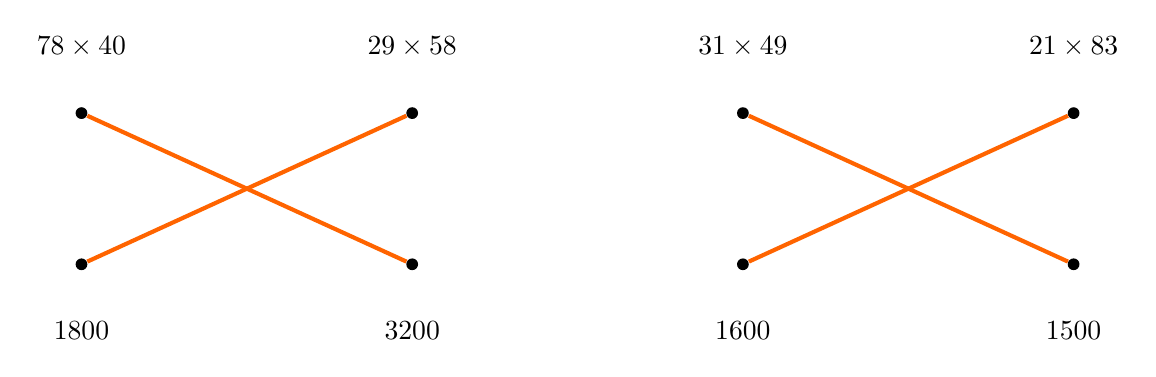
\begin{tikzpicture}[scale=1.2, >=Stealth]
  % 定义颜色
  \definecolor{matchline}{RGB}{255,100,0}

  % 第一部分：算式 (Top row)
  \node (e1) at (0, 3) {$78 \times 40$};
  \node (e2) at (3.5, 3) {$29 \times 58$};
  \node (e3) at (7, 3) {$31 \times 49$};
  \node (e4) at (10.5, 3) {$21 \times 83$};

  % 第一排圆点
  \node[circle, fill, inner sep=1.5pt] (p1) at (0, 2.3) {};
  \node[circle, fill, inner sep=1.5pt] (p2) at (3.5, 2.3) {};
  \node[circle, fill, inner sep=1.5pt] (p3) at (7, 2.3) {};
  \node[circle, fill, inner sep=1.5pt] (p4) at (10.5, 2.3) {};

  % 第二排圆点
  \node[circle, fill, inner sep=1.5pt] (q1) at (0, 0.7) {};
  \node[circle, fill, inner sep=1.5pt] (q2) at (3.5, 0.7) {};
  \node[circle, fill, inner sep=1.5pt] (q3) at (7, 0.7) {};
  \node[circle, fill, inner sep=1.5pt] (q4) at (10.5, 0.7) {};

  % 第二部分：估算结果 (Bottom row)
  \node (r1) at (0, 0) {$1800$};
  \node (r2) at (3.5, 0) {$3200$};
  \node (r3) at (7, 0) {$1600$};
  \node (r4) at (10.5, 0) {$1500$};

  % 连线 (Matching)
  \draw[line width=1.5pt, matchline] (p1) -- (q2); % 78*40 -> 3200
  \draw[line width=1.5pt, matchline] (p2) -- (q1); % 29*58 -> 1800
  \draw[line width=1.5pt, matchline] (p3) -- (q4); % 31*49 -> 1500
  \draw[line width=1.5pt, matchline] (p4) -- (q3); % 21*83 -> 1600

\end{tikzpicture}
\end{center}

\vspace{1.2cm}
\hrule
\vspace{0.4cm}


%% ==============================
%% 行程问题：家、超市与学校
%% ==============================
\newpage

\begin{center}
  {\large\bfseries 解答：行程问题解析图}
\end{center}

\vspace{0.6cm}

\noindent
\begin{center}
\begin{tikzpicture}[scale=0.45, >=Stealth, line width=1pt]
  % 定义颜色
  \definecolor{pathblue}{RGB}{0,191,255}

  % 坐标点定义
  \coordinate (Home) at (0, 0);          % 方华家
  \coordinate (Supermarket) at (-10, 0); % 超市 (1000m -> 10单位)
  \coordinate (School) at (0, 20);      % 学校 (2000m -> 20单位)

  % 绘制路线
  \draw[pathblue, line width=2pt] (Supermarket) -- (Home) -- (School);

  % 绘制各地点标识圆圈
  \filldraw[white, draw=pathblue, line width=1.5pt] (Home) circle (0.6);
  \filldraw[white, draw=pathblue, line width=1.5pt] (Supermarket) circle (0.6);
  \filldraw[white, draw=pathblue, line width=1.5pt] (School) circle (0.6);

  % 地点文字标注
  \node[right=8pt] at (Home) {方华家};
  \node[below=8pt] at (Supermarket) {超市};
  \node[right=8pt] at (School) {学校};

  % % 原始距离标注 (大括号)
  % \draw[decorate, decoration={brace, amplitude=10pt, raise=15pt}]
  %   (Home) -- (Supermarket) node[midway, above=28pt] {1000米};

  % \draw[decorate, decoration={brace, amplitude=10pt, raise=15pt, mirror}]
  %   (Home) -- (School) node[midway, right=28pt] {2000米};

  % --- 第(1)问标注 ---
  % 计算位置：5分钟 * 60米/分 = 300米 -> 3单位 (向超市方向，即水平向左)
  \coordinate (Now) at (-3, 0);
  \node[red, font=\Large] at (Now) {$\bigstar$};
  \node[red, above=10pt, font=\small] at (Now) {现在位置 (300米)};

  % 剩余距离标注
  \draw[<->, red!70!black, line width=0.8pt] (-3.6, -1) -- (-9.4, -1)
    node[midway, below] {\small 剩余700米};

\end{tikzpicture}
\end{center}

\vspace{1.2cm}
\hrule
\vspace{0.4cm}

{\small\color{gray}
\textbf{解析文字：}\\
\textcircled{1} \textbf{计算现在位置：}\\
速度 $60 \times$ 时间 $5 = 300$（米）。\\
方华现在距离家 $300$ 米，在去超市的路上（见图中 $\bigstar$ 标识）。\\
离超市还有：$1000 - 300 = 700$（米）。

\vspace{0.3cm}
\textcircled{2} \textbf{判断能否走到学校：}\\
走 $35$ 分钟的路程：$60 \times 35 = 2100$（米）。\\
由于家到学校的距离是 $2000$ 米，$2100 > 2000$，\\
所以他\textbf{能}走到学校，并且超过了 $100$ 米。
}


%% ==============================
%% 找规律接着画一画
%% ==============================
\newpage

\begin{center}
  {\large\bfseries 解答：按照规律接着画一画}
\end{center}

\vspace{0.4cm}

% 定义常用图形命令
\newcommand{\tikzTriangle}[1]{% 空心/实心三角形
  \begin{tikzpicture}[baseline=-0.8ex]
    \draw[line width=0.8pt, #1] (0,0) -- (0.4,0) -- (0.2,0.35) -- cycle;
  \end{tikzpicture}%
}
\newcommand{\tikzCircle}[1]{% 圆形
  \begin{tikzpicture}[baseline=-0.8ex]
    \draw[line width=0.8pt, #1] (0.15,0.15) circle (0.18);
  \end{tikzpicture}%
}
\newcommand{\tikzSquare}[1]{% 正方形
  \begin{tikzpicture}[baseline=-0.8ex]
    \draw[line width=0.8pt, #1] (0,0) rectangle (0.35,0.35);
  \end{tikzpicture}%
}
\newcommand{\tikzStar}[1]{% 星形
  \begin{tikzpicture}[baseline=-0.8ex]
    \node[#1, inner sep=0pt, font=\large] at (0,0.1) {$\bigstar$};
  \end{tikzpicture}%
}
\newcommand{\tikzSolidStar}[1]{% 实心星
  \begin{tikzpicture}[baseline=-0.8ex]
    \node[#1, inner sep=0pt, font=\large] at (0,0.1) {$\blackstar$};
  \end{tikzpicture}%
}
\newcommand{\tikzSolidTriangle}[1]{% 实心三角
  \begin{tikzpicture}[baseline=-0.8ex]
    \fill[#1] (0,0) -- (0.4,0) -- (0.2,0.35) -- cycle;
  \end{tikzpicture}%
}

\vspace{0.6cm}

\noindent
(1) \tikzTriangle{} \tikzCircle{} \tikzSquare{} \tikzTriangle{} \tikzCircle{} \tikzSquare{} \tikzTriangle{} \tikzCircle{} (\tikzSquare{red!70!black}) (\tikzTriangle{red!70!black}) ……

\vspace{0.8cm}

\noindent
(2) \tikzSquare{} \tikzSquare{} \tikzCircle{} \tikzTriangle{} \tikzSquare{} \tikzSquare{} \tikzCircle{} \tikzTriangle{} \tikzSquare{} (\tikzSquare{red!70!black}) \tikzCircle{} (\tikzTriangle{red!70!black}) ……

\vspace{0.8cm}

\noindent
(3) \tikzSolidTriangle{} \tikzStar{} \tikzStar{} \tikzSolidTriangle{} \tikzSolidTriangle{} \tikzSolidTriangle{} \tikzSolidTriangle{} \tikzStar{} \tikzStar{} \tikzSolidTriangle{} \tikzStar{} (\tikzStar{red!70!black}) (\tikzSolidTriangle{red!70!black}) (\tikzSolidTriangle{red!70!black}) \tikzStar{} (\tikzSolidTriangle{red!70!black}) ……

\vspace{1.2cm}
\hrule
\vspace{0.4cm}

{\small\color{gray}
\textbf{规律分析：}\\
\textcircled{1} \textbf{第(1)题：}观察可知，图形是以 \tikzTriangle{} \tikzCircle{} \tikzSquare{} 为一组循环出现的。前面已有 \tikzTriangle{} \tikzCircle{}，按照顺序，接下来应填 \tikzSquare{} 和 \tikzTriangle{}。

\vspace{0.3cm}
\textcircled{2} \textbf{第(2)题：}观察可知，图形是以 \tikzSquare{} \tikzSquare{} \tikzCircle{} \tikzTriangle{} 为一组循环出现的。空格前为 \tikzSquare{}，接下来的序列缺第二个 \tikzSquare{}，因此第一个括号填 \tikzSquare{}，跳过已有的 \tikzCircle{}，第二个括号填 \tikzTriangle{}。

\vspace{0.3cm}
\textcircled{3} \textbf{第(3)题：}该组图形由 \tikzSolidTriangle{} \tikzStar{} \tikzStar{} 和 \tikzSolidTriangle{} \tikzSolidTriangle{} \tikzSolidTriangle{} 两组交替出现。根据现有序列末尾的 \tikzSolidTriangle{} \tikzStar{}，需先补完 \tikzStar{} 构成第一组，随后补完 \tikzSolidTriangle{} \tikzSolidTriangle{} \tikzSolidTriangle{} 构成第二组。故依次填入：\tikzStar{}、\tikzSolidTriangle{}、\tikzSolidTriangle{}、\tikzSolidTriangle{}。
}


%% ==============================
%% 球类爱好项目统计
%% ==============================
\newpage

\begin{center}
  {\large\bfseries 解答：四(2)班球类爱好项目统计}
\end{center}

\vspace{0.4cm}

% 1. 统计表
\begin{center}
  {\small 四(2)班球类爱好项目统计表} \\
  \vspace{0.2cm}
  \renewcommand{\arraystretch}{1.5}
  \begin{tabular}{|c|c|c|c|c|c|}
    \hline
    项目类别 & 合计 & 排球 & 足球 & 篮球 & 乒乓球 \\
    \hline
    人数 & \textbf{\textcolor{red!70!black}{45}} & 8 & 20 & 12 & 5 \\
    \hline
  \end{tabular}
\end{center}

\vspace{0.8cm}

% 2. 条形统计图
\begin{center}
  {\small 四(2)班球类爱好项目统计图} \\
  \vspace{0.4cm}
  \begin{tikzpicture}[xscale=1.5, yscale=0.15, >=Stealth]
    % 绘图参数：1单位高度 = 1人
    
    % 分格线与纵轴坐标
    \foreach \y in {5,10,...,30} {
      \draw[gray!30, line width=0.5pt] (0, \y) -- (8.5, \y);
      \node[left, font=\footnotesize] at (0, \y) {\y};
    }
    \node[left, font=\footnotesize] at (0, 0) {0};
    \foreach \x in {0,1,...,8} {
      \draw[gray!30, line width=0.5pt] (\x, 0) -- (\x, 30);
    }
    \node[above left, font=\footnotesize] at (0, 31) {人数/人};
    
    % 纵横轴
    \draw[->, line width=0.8pt] (0, 0) -- (0, 33);
    \draw[->, line width=0.8pt] (0, 0) -- (9, 0) node[right, font=\footnotesize] {项目类别};
    
    % 绘制条形 (每个条形宽1单位)
    % 排球: 8人
    \filldraw[fill=blue!50!cyan!70, draw=blue!50!black] (1,0) rectangle (2, 8);
    \node[below, font=\small] at (1.5, 0) {排球};
    \node[above, font=\scriptsize, blue!50!black] at (1.5, 8) {8};
    
    % 足球: 20人
    \filldraw[fill=blue!50!cyan!70, draw=blue!50!black] (3,0) rectangle (4, 20);
    \node[below, font=\small] at (3.5, 0) {足球};
    \node[above, font=\scriptsize, blue!50!black] at (3.5, 20) {20};
    
    % 篮球: 12人
    \filldraw[fill=blue!50!cyan!70, draw=blue!50!black] (5,0) rectangle (6, 12);
    \node[below, font=\small] at (5.5, 0) {篮球};
    \node[above, font=\scriptsize, blue!50!black] at (5.5, 12) {12};
    
    % 乒乓球: 5人
    \filldraw[fill=blue!50!cyan!70, draw=blue!50!black] (7,0) rectangle (8, 5);
    \node[below, font=\small] at (7.5, 0) {乒乓球};
    \node[above, font=\scriptsize, blue!50!black] at (7.5, 5) {5};

  \end{tikzpicture}
\end{center}

\vspace{1.0cm}
\hrule
\vspace{0.4cm}

% 3. 问题解答
{\small
  (1) 条形统计图中纵轴上每格表示(\ \textbf{\textcolor{red!70!black}{5}}\ )人。 \\
  \vspace{0.2cm}
  (2) 四(2)班爱好(\ \textbf{\textcolor{red!70!black}{足球}}\ )项目的人数最多，爱好(\ \textbf{\textcolor{red!70!black}{乒乓球}}\ )的项目人数最少。 \\
  \vspace{0.2cm}
  (3) 四(2)班爱好乒乓球的比爱好篮球的少(\ \textbf{\textcolor{red!70!black}{7}}\ )人。 ($12 - 5 = 7$) \\
  \vspace{0.2cm}
  (4) 四(2)班学生一共有(\ \textbf{\textcolor{red!70!black}{45}}\ )人。 ($8 + 20 + 12 + 5 = 45$)
}


%% ==============================
%% 地铁站乘坐地铁不同付款方式人数统计
%% ==============================
\newpage

\begin{center}
  {\large\bfseries 解答：地铁站某时段乘坐地铁各付款方式人数统计}
\end{center}

\vspace{0.4cm}

% 1. 统计表
\begin{center}
  \renewcommand{\arraystretch}{1.5}
  \begin{tabular}{|c|c|c|c|c|}
    \hline
    付款方式 & 地铁票 & 刷银行卡 & 扫乘车码 & 专用 App \\
    \hline
    人数 & 150 & 240 & 300 & 320 \\
    \hline
  \end{tabular}
\end{center}

\vspace{0.8cm}

% 2. 条形统计图
\begin{center}
  {\small 某地铁站某时段乘坐地铁不同付款方式的人数统计图} \\
  \vspace{0.4cm}
  \begin{tikzpicture}[xscale=1.4, yscale=0.02, >=Stealth]
    % 绘图参数：1单位高度 = 1人，每50人一格，纵轴显示到 350
    
    % 背景网格 (x从0到8.5, y从0到350)
    \foreach \y in {50,100,...,350} {
      \draw[gray!30, line width=0.5pt] (0, \y) -- (8.5, \y);
      \node[left, font=\footnotesize] at (0, \y) {\y};
    }
    \foreach \x in {0,1,...,8} {
      \draw[gray!30, line width=0.5pt] (\x, 0) -- (\x, 350);
    }
    
    % 纵横轴
    \draw[->, line width=0.8pt] (0, 0) -- (0, 380) node[above, font=\footnotesize] {人数/人};
    \draw[->, line width=0.8pt] (0, 0) -- (9, 0) node[right, font=\footnotesize] {付款方式};
    \node[below left, font=\footnotesize] at (0,0) {0};
    
    % 绘制条形 (每个条形宽1单位, 对齐网格 1-2, 3-4, 5-6, 7-8)
    % 地铁票: 150
    \filldraw[fill=blue!50!cyan!70, draw=blue!50!black] (1,0) rectangle (2, 150);
    \node[below, font=\small] at (1.5, 0) {地铁票};
    
    % 刷银行卡: 240
    \filldraw[fill=blue!50!cyan!70, draw=blue!50!black] (3,0) rectangle (4, 240);
    \node[below, font=\small] at (3.5, 0) {刷银行卡};
    
    % 扫乘车码: 300
    \filldraw[fill=blue!50!cyan!70, draw=blue!50!black] (5,0) rectangle (6, 300);
    \node[below, font=\small] at (5.5, 0) {扫乘车码};
    
    % 专用 App: 320
    \filldraw[fill=blue!50!cyan!70, draw=blue!50!black] (7,0) rectangle (8, 320);
    \node[below, font=\small] at (7.5, 0) {专用 App};

  \end{tikzpicture}
\end{center}

\vspace{1.0cm}
\hrule
\vspace{0.4cm}

% 3. 问题解答
{\small
  (1) 如果用条形统计图表示上面的数据，1 格代表(\ \textbf{\textcolor{red!70!black}{50}}\ )人比较合适。 \\
  \vspace{0.3cm}
  (2) 绘图解析：如上图所示，地铁票对应 3 格高度，刷银行卡对应 4.8 格高度，扫乘车码对应 6 格高度，专用 App 对应 6.4 格高度。 \\
}


%% ==============================
%% 六(1)班男生体测成绩统计
%% ==============================
\newpage

\begin{center}
  {\large\bfseries 解答：六(1)班男生体育测试成绩统计}
\end{center}

\vspace{0.4cm}

% 1. 统计表
\begin{center}
  {\small 实验小学六(1)班男生体育测试成绩统计表} \\
  \vspace{0.2cm}
  \renewcommand{\arraystretch}{1.5}
  \begin{tabular}{|c|c|c|c|c|c|}
    \hline
    成绩 & 合计 & 优秀 & 良好 & 合格 & 不合格 \\
    \hline
    人数 & \textbf{\textcolor{red!70!black}{20}} & 3 & 8 & 8 & 1 \\
    \hline
  \end{tabular}
\end{center}

\vspace{0.8cm}

% 2. 条形统计图
\begin{center}
  {\small 实验小学六(1)班男生体育测试成绩统计图} \\
  \vspace{0.4cm}
  \begin{tikzpicture}[xscale=1.6, yscale=0.5, >=Stealth]
    % 纵轴：每格表示2人，最高14
    
    % 背景网格
    \foreach \y in {2,4,...,14} {
      \draw[gray!30, line width=0.5pt] (0, \y) -- (8.5, \y);
      \node[left, font=\footnotesize] at (0, \y) {\y};
    }
    \node[left, font=\footnotesize] at (0, 0) {0};
    \foreach \x in {0,1,...,8} {
      \draw[gray!30, line width=0.5pt] (\x, 0) -- (\x, 14);
    }
    
    % 纵横轴
    \draw[->, line width=0.8pt] (0, 0) -- (0, 15.5) node[above, font=\footnotesize] {人数/人};
    \draw[->, line width=0.8pt] (0, 0) -- (9, 0) node[right, font=\footnotesize] {成绩};
    
    % 绘制条形 (柱宽1)
    % 优秀: 3人
    \filldraw[fill=blue!50!cyan!70, draw=blue!50!black] (1, 0) rectangle (2, 3);
    \node[below, font=\small] at (1.5, 0) {优秀};
    \node[above, font=\scriptsize, blue!50!black] at (1.5, 3) {3};
    
    % 良好: 8人
    \filldraw[fill=blue!50!cyan!70, draw=blue!50!black] (3, 0) rectangle (4, 8);
    \node[below, font=\small] at (3.5, 0) {良好};
    \node[above, font=\scriptsize, blue!50!black] at (3.5, 8) {8};
    
    % 合格: 8人
    \filldraw[fill=blue!50!cyan!70, draw=blue!50!black] (5, 0) rectangle (6, 8);
    \node[below, font=\small] at (5.5, 0) {合格};
    \node[above, font=\scriptsize, blue!50!black] at (5.5, 8) {8};
    
    % 不合格: 1人
    \filldraw[fill=blue!50!cyan!70, draw=blue!50!black] (7, 0) rectangle (8, 1);
    \node[below, font=\small] at (7.5, 0) {不合格};
    \node[above, font=\scriptsize, blue!50!black] at (7.5, 1) {1};

  \end{tikzpicture}
\end{center}

\vspace{1.0cm}
\hrule
\vspace{0.4cm}

% 3. 问题解答
{\small
  (1) 这个班有男生(\ \textbf{\textcolor{red!70!black}{20}}\ )人。 \\
  \vspace{0.2cm}
  (2) 从表格中可以看出，体育测试成绩(\ \textbf{\textcolor{red!70!black}{不合格}}\ )的人数最少，\\
  \quad\quad (\ \textbf{\textcolor{red!70!black}{良好}}\ )和(\ \textbf{\textcolor{red!70!black}{合格}}\ )的人数一样多。
}


%% ==============================
%% 四(2)班女生2分钟口算成绩统计
%% ==============================
\newpage

\begin{center}
  {\large\bfseries 解答：四(2)班女生 2 分钟口算成绩统计}
\end{center}

\vspace{0.4cm}

% 1. 统计表
\begin{center}
  {\small 四(2)班女生 2 分钟口算成绩统计表} \\
  \vspace{0.2cm}
  \renewcommand{\arraystretch}{1.5}
  \begin{tabular}{|c|c|c|c|c|c|}
    \hline
    答对题数 & 合计 & 30～39 & 40～49 & 50～59 & 60～69 \\
    \hline
    人数 & \textbf{\textcolor{red!70!black}{20}} & 1 & 8 & 7 & 4 \\
    \hline
  \end{tabular}
\end{center}

\vspace{0.8cm}

% 2. 条形统计图
\begin{center}
  {\small 四(2)班女生 2 分钟口算成绩统计图} \\
  \vspace{0.4cm}
  \begin{tikzpicture}[xscale=1.6, yscale=0.5, >=Stealth]
    % 纵轴：每格表示2人，最高12
    
    % 背景网格 (x: 0-8, y: 0-12)
    \foreach \y in {2,4,...,12} {
      \draw[gray!30, line width=0.5pt] (0, \y) -- (8.5, \y);
      \node[left, font=\footnotesize] at (0, \y) {\y};
    }
    \node[left, font=\footnotesize] at (0, 0) {0};
    \foreach \x in {0,1,...,8} {
      \draw[gray!30, line width=0.5pt] (\x, 0) -- (\x, 12);
    }
    
    % 纵横轴
    \draw[->, line width=0.8pt] (0, 0) -- (0, 13) node[above, font=\footnotesize] {人数/人};
    \draw[->, line width=0.8pt] (0, 0) -- (9, 0) node[right, font=\footnotesize] {答对题数};
    
    % 绘制条形 (柱宽1)
    % 30~39: 1人
    \filldraw[fill=blue!50!cyan!70, draw=blue!50!black] (1, 0) rectangle (2, 1);
    \node[below, font=\small] at (1.5, 0) {30～39};
    \node[above, font=\scriptsize, blue!50!black] at (1.5, 1) {1};
    
    % 40~49: 8人
    \filldraw[fill=blue!50!cyan!70, draw=blue!50!black] (3, 0) rectangle (4, 8);
    \node[below, font=\small] at (3.5, 0) {40～49};
    \node[above, font=\scriptsize, blue!50!black] at (3.5, 8) {8};
    
    % 50~59: 7人
    \filldraw[fill=blue!50!cyan!70, draw=blue!50!black] (5, 0) rectangle (6, 7);
    \node[below, font=\small] at (5.5, 0) {50～59};
    \node[above, font=\scriptsize, blue!50!black] at (5.5, 7) {7};
    
    % 60~69: 4人
    \filldraw[fill=blue!50!cyan!70, draw=blue!50!black] (7, 0) rectangle (8, 4);
    \node[below, font=\small] at (7.5, 0) {60～69};
    \node[above, font=\scriptsize, blue!50!black] at (7.5, 4) {4};

  \end{tikzpicture}
\end{center}

\vspace{1.0cm}
\hrule
\vspace{0.4cm}

% 3. 问题解答
{\small
  (2) 四(2)班女生 2 分钟口算答对题数在(\ \textbf{\textcolor{red!70!black}{$40 \sim 49$}}\ )的人数最多。 \\
  \vspace{0.3cm}
  (3) 小红的成绩在全班女生中排第五名。我们按成绩从高到低排列： \\
  \textbf{67, 65, 61, 60}, \textcolor{red!70!black}{58}, 57, 56, 55, 52, 51, 50, 48, 47, 45, 44, 43, 42, 41, 40, 36。 \\
  第五名对应的分数是(\ \textbf{\textcolor{red!70!black}{58}}\ )。
}


%% ==============================
%% 文文、小玲和小青书签枚数统计
%% ==============================
\newpage

\begin{center}
  {\large\bfseries 解答：文文、小玲和小青书签枚数统计}
\end{center}

\vspace{0.4cm}

% 逻辑分析说明
{\small
\textbf{逻辑解析：} \\
1. 从图中的格数看：文文占 9 格，小玲占 2 格，小青占 4 格，总格数为 $9 + 2 + 4 = 15$ 格。 \\
2. 三人书签数一样多时，每人应有 $15 \div 3 = 5$ 格。 \\
3. 文文拿出 40 枚分给其他两人后三人相等，意味着文文从 9 格减少到 5 格，减少的这 4 格对应 40 枚。 \\
4. 因此，\textbf{1 格代表 $40 \div 4 = 10$ 枚书签}。
}

\vspace{0.6cm}

% 1. 统计图
\begin{center}
  {\small 文文、小玲、小青书签枚数统计图} \\
  \vspace{0.4cm}
  \begin{tikzpicture}[xscale=1.0, yscale=0.1, >=Stealth]
    % 纵轴：1格（10枚）对应 1cm，横轴 1单位对应 1cm
    
    % 背景网格
    \foreach \y in {10,20,...,100} {
      \draw[gray!30, line width=0.5pt] (0, \y) -- (8, \y);
      \node[left, font=\footnotesize] at (0, \y) {\y};
    }
    \node[left, font=\footnotesize] at (0, 0) {0};
    \foreach \x in {0,1,...,8} {
      \draw[gray!30, line width=0.5pt] (\x, 0) -- (\x, 100);
    }
    
    % 纵横轴
    \draw[->, line width=0.8pt] (0, 0) -- (0, 110) node[above, font=\footnotesize] {书签/枚};
    \draw[->, line width=0.8pt] (0, 0) -- (8.5, 0);
    
    % 绘制条形 (柱宽1, 对齐网格 1-2, 3-4, 5-6)
    % 文文: 9格 = 90枚
    \filldraw[fill=blue!50!cyan!70, draw=blue!50!black] (1, 0) rectangle (2, 90);
    \node[below, font=\small] at (1.5, 0) {文文};
    \node[above, font=\scriptsize, blue!50!black] at (1.5, 90) {( 90 )};
    
    % 小玲: 2格 = 20枚
    \filldraw[fill=blue!50!cyan!70, draw=blue!50!black] (3, 0) rectangle (4, 20);
    \node[below, font=\small] at (3.5, 0) {小玲};
    \node[above, font=\scriptsize, blue!50!black] at (3.5, 20) {( 20 )};
    
    % 小青: 4格 = 40枚
    \filldraw[fill=blue!50!cyan!70, draw=blue!50!black] (5, 0) rectangle (6, 40);
    \node[below, font=\small] at (5.5, 0) {小青};
    \node[above, font=\scriptsize, blue!50!black] at (5.5, 40) {( 40 )};

  \end{tikzpicture}
\end{center}

\vspace{0.8cm}
\hrule
\vspace{0.4cm}

% 2. 问题解答
{\small
  (1) \textbf{填写完善统计图：} 如上图所示，纵轴刻度依次为 10, 20, ..., 100；柱状图上方数值分别为 90, 20, 40。 \\
  \vspace{0.3cm}
  (2) 如果亮亮的书签枚数在图中正好画 5 格，那么亮亮有(\ \textbf{\textcolor{red!70!black}{50}}\ )枚书签。 ($5 \times 10 = 50$)
}


%% ==============================
%% 五角星和六角星数量统计
%% ==============================
\newpage

\begin{center}
  {\large\bfseries 解答：五角星和六角星数量统计}
\end{center}

\vspace{0.4cm}

% 定义本页特定图形宏
\newcommand{\tikzFiveStarStat}{%
  
\begin{tikzpicture}[baseline=-0.5ex, scale=0.15]
    \draw[cyan!70!blue, thick] (90:1) -- (234:1) -- (18:1) -- (162:1) -- (306:1) -- cycle;
  \end{tikzpicture}%
}
\newcommand{\tikzSixStarStat}{%
  
\begin{tikzpicture}[baseline=-0.5ex, scale=0.15]
    \draw[cyan!70!blue, thick] (90:1) -- (210:1) -- (330:1) -- cycle;
    \draw[cyan!70!blue, thick] (270:1) -- (30:1) -- (150:1) -- cycle;
  \end{tikzpicture}%
}

\noindent
{\small
\textbf{数据统计逻辑：} \\
通过观察图中的排列规律（三角形阵列）： \\
$\bullet$ 第 1, 3, 5 行是五角星 \tikzFiveStarStat{}，数量分别为 1, 3, 5 个，合计 $1 + 3 + 5 = 9$ 个。 \\
$\bullet$ 第 2, 4 行是六角星 \tikzSixStarStat{}，数量分别为 2, 4 个，合计 $2 + 4 = 6$ 个。 \\
$\bullet$ 总计：$9 + 6 = 15$ 个。
}

\vspace{0.6cm}

% 1. 统计表
\begin{center}
  \renewcommand{\arraystretch}{1.5}
  \begin{tabular}{|c|c|c|c|}
    \hline
    形状 & 合计 & 五角星 & 六角星 \\
    \hline
    个数 & \textbf{\textcolor{red!70!black}{15}} & 9 & 6 \\
    \hline
  \end{tabular}
\end{center}

\vspace{0.8cm}

% 2. 条形统计图
\begin{center}
  {\small 五角星和六角星数量统计图} \\
  \vspace{0.4cm}
  \begin{tikzpicture}[xscale=1.0, yscale=0.5, >=Stealth]
    % 纵轴：2个对应 1cm，横轴 1单位对应 1cm
    
    % 背景网格
    \foreach \y in {2,4,6,8,10,12,14} {
      \draw[gray!30, line width=0.5pt] (0, \y) -- (6, \y);
      \node[left, font=\footnotesize] at (0, \y) {\y};
    }
    \node[left, font=\footnotesize] at (0, 0) {0};
    \foreach \x in {0,1,...,6} {
      \draw[gray!30, line width=0.5pt] (\x, 0) -- (\x, 14);
    }
    
    % 纵横轴
    \draw[->, line width=0.8pt] (0, 0) -- (0, 15.5) node[above, font=\footnotesize] {数量/个};
    \draw[->, line width=0.8pt] (0, 0) -- (6.5, 0);
    
    % 绘制条形 (柱宽1, 对齐网格 1-2, 3-4)
    % 五角星: 9个
    \filldraw[fill=blue!50!cyan!70, draw=blue!50!black] (1, 0) rectangle (2, 9);
    \node[below, font=\small] at (1.5, 0) {五角星};
    \node[above, font=\scriptsize, blue!50!black] at (1.5, 9) {9};
    
    % 六角星: 6个
    \filldraw[fill=blue!50!cyan!70, draw=blue!50!black] (3, 0) rectangle (4, 6);
    \node[below, font=\small] at (3.5, 0) {六角星};
    \node[above, font=\scriptsize, blue!50!black] at (3.5, 6) {6};

  \end{tikzpicture}
\end{center}

\vspace{1.0cm}
\hrule
\vspace{0.4cm}

% 3. 问题解答
{\small
  (1) \textbf{填写统计图表：} 统计表中填入合计 15，五角星 9，六角星 6。统计图中纵轴刻度由下至上标为 0, 2, 4, 6, 8, 10, 12, 14。 \\
  \vspace{0.3cm}
  (2) 根据条形统计图可知，五角星共有 9 个，六角星共有 6 个，总数共 15 个。
}


%% ==============================
%% 四(1)班男生1分钟跳绳成绩统计
%% ==============================
\newpage

\begin{center}
  {\large\bfseries 解答：四(1)班男生1分钟跳绳成绩统计}
\end{center}

\vspace{0.4cm}

% 数据整理与逻辑分析
{\small
\textbf{数据整理：} \\
1. \textbf{成绩原始记录：} 56, 41, 116, 117, 120, 138, 125, 39, 132, 124, 94, 106, 98, 121, 42, 77, 72, 122, 135, 38, 40, 123, 41, 126。 \\
2. \textbf{统计分类标准：} \\
   $\bullet$ 优秀（$>126$次）：138, 132, 135，共 \textbf{3} 人。 \\
   $\bullet$ 良好（$115 \sim 126$次）：116, 117, 120, 125, 124, 121, 122, 123, 126，共 \textbf{9} 人。 \\
   $\bullet$ 合格（$45 \sim 114$次）：56, 94, 106, 98, 77, 72，共 \textbf{6} 人。 \\
   $\bullet$ 不合格（$<45$次）：41, 39, 42, 38, 40, 41，共 \textbf{6} 人。 \\
3. \textbf{总人数：} $3 + 9 + 6 + 6 = 24$ 人。
}

\vspace{0.6cm}

% 1. 统计表
\begin{center}
  {\small 四(1)班男生1分钟跳绳等级统计表} \\
  \vspace{0.2cm}
  \renewcommand{\arraystretch}{1.5}
  \begin{tabular}{|c|c|c|c|c|c|}
    \hline
    等级 & 合计 & 优秀 & 良好 & 合格 & 不合格 \\
    \hline
    人数 & \textbf{\textcolor{red!70!black}{24}} & \textbf{\textcolor{red!70!black}{3}} & \textbf{\textcolor{red!70!black}{9}} & \textbf{\textcolor{red!70!black}{6}} & \textbf{\textcolor{red!70!black}{6}} \\
    \hline
  \end{tabular}
\end{center}

\vspace{0.8cm}

% 2. 条形统计图
\begin{center}
  {\small 四(1)班男生1分钟跳绳成绩等级统计图} \\
  \vspace{0.4cm}
  \begin{tikzpicture}[xscale=1.0, yscale=0.5, >=Stealth]
    % 纵轴：2人对应 1cm，横轴 1单位对应 1cm
    \foreach \y in {2,4,6,8,10} {
      \draw[gray!30, line width=0.5pt] (0, \y) -- (8, \y);
      \node[left, font=\footnotesize] at (0, \y) {\y};
    }
    \foreach \x in {0,1,...,8} {
      \draw[gray!30, line width=0.5pt] (\x, 0) -- (\x, 10);
    }
    \node[left, font=\footnotesize] at (0, 0) {0};
    
    % 纵横轴
    \draw[->, line width=0.8pt] (0, 0) -- (0, 11) node[above, font=\footnotesize] {人数/人};
    \draw[->, line width=0.8pt] (0, 0) -- (8.5, 0);
    
    % 绘制条形
    % 优秀: 3人
    \filldraw[fill=blue!40!cyan!60, draw=blue!50!black] (1, 0) rectangle (2, 3);
    \node[below, font=\small] at (1.5, 0) {优秀};
    \node[above, font=\scriptsize, blue!50!black] at (1.5, 3) {3};
    
    % 良好: 9人
    \filldraw[fill=blue!40!cyan!60, draw=blue!50!black] (3, 0) rectangle (4, 9);
    \node[below, font=\small] at (3.5, 0) {良好};
    \node[above, font=\scriptsize, blue!50!black] at (3.5, 9) {9};
    
    % 合格: 6人
    \filldraw[fill=blue!40!cyan!60, draw=blue!50!black] (5, 0) rectangle (6, 6);
    \node[below, font=\small] at (5.5, 0) {合格};
    \node[above, font=\scriptsize, blue!50!black] at (5.5, 6) {6};
    
    % 不合格: 6人
    \filldraw[fill=blue!40!cyan!60, draw=blue!50!black] (7, 0) rectangle (8, 6);
    \node[below, font=\small] at (7.5, 0) {不合格};
    \node[above, font=\scriptsize, blue!50!black] at (7.5, 6) {6};

  \end{tikzpicture}
\end{center}

\vspace{0.8cm}
\hrule
\vspace{0.4cm}

% 3. 问题解答
{\small
  (2) 这个班男生 1 分钟跳绳的最好成绩是(\ \textbf{\textcolor{red!70!black}{138}}\ )次，最差成绩是(\ \textbf{\textcolor{red!70!black}{38}}\ )次。 \\
  \vspace{0.3cm}
  (3) 这个班男生 1 分钟跳绳等级为(\ \textbf{\textcolor{red!70!black}{良好}}\ )的人数最多，等级为(\ \textbf{\textcolor{red!70!black}{优秀}}\ )的人数最少，两者相差(\ \textbf{\textcolor{red!70!black}{6}}\ )人。 ($9 - 3 = 6$)
}


%% ==============================
%% 晓辉家的生活垃圾分类情况统计
%% ==============================
\newpage

\begin{center}
  {\large\bfseries 解答：晓辉家的生活垃圾分类情况统计}
\end{center}

\vspace{0.4cm}

% 数据分类逻辑分析
{\small
\textbf{数据分类整理：} \\
根据《江苏省城市生活垃圾分类设施设备配置和维护指南》，分类如下： \\
1. \textbf{可回收物：} 废旧报纸 ($900$克) + 矿泉水瓶 ($400$克) + 旧的衣服 ($1100$克) = \textbf{2400} 克。 \\
2. \textbf{有害垃圾：} 废弃铅蓄电池 ($500$克) + 过期药品 ($100$克) = \textbf{600} 克。 \\
3. \textbf{厨余垃圾：} 剩饭剩菜 = \textbf{1200} 克。 \\
4. \textbf{其他垃圾：} 陶瓷碎片 = \textbf{1000} 克。 \\
\textbf{总计：} $2400 + 600 + 1200 + 1000 = 5200$ 克。
}

\vspace{0.6cm}

% 1. 统计表
\begin{center}
  {\small 晓辉家的生活垃圾分类情况统计表} \\
  \vspace{0.2cm}
  \renewcommand{\arraystretch}{1.5}
  \begin{tabular}{|c|c|c|c|c|}
    \hline
    垃圾类别 & 可回收物 & 有害垃圾 & 厨余垃圾 & 其他垃圾 \\
    \hline
    质量/克 & \textbf{\textcolor{red!70!black}{2400}} & \textbf{\textcolor{red!70!black}{600}} & \textbf{\textcolor{red!70!black}{1200}} & \textbf{\textcolor{red!70!black}{1000}} \\
    \hline
  \end{tabular}
\end{center}

\vspace{0.8cm}

% 2. 条形统计图
\begin{center}
  {\small 晓辉家的生活垃圾分类情况统计图} \\
  \vspace{0.4cm}
  \begin{tikzpicture}[xscale=1.0, yscale=2.5, >=Stealth]
    % 纵轴：400克对应 1cm (0.4 * 2.5), 横轴 1单位对应 1cm
    \foreach \y in {400,800,1200,1600,2000,2400,2800} {
      \draw[gray!30, line width=0.5pt] (0, \y/1000) -- (8, \y/1000);
      \node[left, font=\footnotesize] at (0, \y/1000) {\y};
    }
    \foreach \x in {0,1,...,8} {
      \draw[gray!30, line width=0.5pt] (\x, 0) -- (\x, 2.8);
    }
    \node[left, font=\footnotesize] at (0, 0) {0};
    
    % 纵横轴
    \draw[->, line width=0.8pt] (0, 0) -- (0, 3.1) node[above, font=\footnotesize] {质量/克};
    \draw[->, line width=0.8pt] (0, 0) -- (8.5, 0);
    
    % 绘制条形
    % 可回收物: 2400克
    \filldraw[fill=blue!40!cyan!60, draw=blue!50!black] (1, 0) rectangle (2, 2.4);
    \node[below, font=\small] at (1.5, 0) {可回收物};
    \node[above, font=\scriptsize, blue!50!black] at (1.5, 2.4) {2400};
    
    % 有害垃圾: 600克
    \filldraw[fill=blue!40!cyan!60, draw=blue!50!black] (3, 0) rectangle (4, 0.6);
    \node[below, font=\small] at (3.5, 0) {有害垃圾};
    \node[above, font=\scriptsize, blue!50!black] at (3.5, 0.6) {600};
    
    % 厨余垃圾: 1200克
    \filldraw[fill=blue!40!cyan!60, draw=blue!50!black] (5, 0) rectangle (6, 1.2);
    \node[below, font=\small] at (5.5, 0) {厨余垃圾};
    \node[above, font=\scriptsize, blue!50!black] at (5.5, 1.2) {1200};
    
    % 其他垃圾: 1000克
    \filldraw[fill=blue!40!cyan!60, draw=blue!50!black] (7, 0) rectangle (8, 1.0);
    \node[below, font=\small] at (7.5, 0) {其他垃圾};
    \node[above, font=\scriptsize, blue!50!black] at (7.5, 1.0) {1000};

  \end{tikzpicture}
\end{center}

\vspace{0.8cm}
\hrule
\vspace{0.4cm}

% 3. 问题解答
{\small
  (2) 晓辉家这段时间积累的(\ \textbf{\textcolor{red!70!black}{可回收物}}\ )垃圾最多，积累的(\ \textbf{\textcolor{red!70!black}{有害垃圾}}\ )垃圾最少。 \\
  \vspace{0.3cm}
  (3) 可回收物比厨余垃圾多(\ \textbf{\textcolor{red!70!black}{1200}}\ )克。 ($2400 - 1200 = 1200$) \\
  \vspace{0.3cm}
  (4) \textbf{建议：} 可以设立分类奖励积分制，用积分兑换生活小礼品，从而提高大家参与垃圾分类的积极性；同时在小区内加强垃圾分类知识的宣传，让每位居民都清楚分类标准。
}


%% ==============================
%% 平行与垂直的练习
%% ==============================
\newpage

\begin{center}
  {\large\bfseries 解答：平行与垂直的练习}
\end{center}

\vspace{0.6cm}

\noindent
{\small \textbf{题目要求：} 在互相平行的两条直线下面画“//”，互相垂直的两条直线下面画“$\perp$”。}

\vspace{0.8cm}

\begin{center}
  \begin{tikzpicture}[scale=1.2, >=Stealth]
    
    %% 第一排
    % 1. 平行 (左倾)
    \begin{scope}[xshift=0cm, yshift=4cm]
      \draw[cyan!70!blue, thick] (-0.8, 1.2) -- (0.8, -0.4);
      \draw[cyan!70!blue, thick] (-0.3, 1.3) -- (1.3, -0.3);
      \node[below] at (0.25, -0.8) {$(\ \textcolor{red!70!black}{/\!/} \ )$};
    \end{scope}

    % 2. 不平行不垂直
    \begin{scope}[xshift=3.5cm, yshift=4cm]
      \draw[cyan!70!blue, thick] (-0.5, 1.3) -- (0.3, -0.3);
      \draw[cyan!70!blue, thick] (1.2, 1.5) -- (1.5, -0.4);
      \node[below] at (0.5, -0.8) {$(\ \ \ )$};
    \end{scope}

    % 3. 平行 (右倾)
    \begin{scope}[xshift=7cm, yshift=4cm]
      \draw[cyan!70!blue, thick] (-0.3, 0.2) -- (1.5, 1.8);
      \draw[cyan!70!blue, thick] (0.2, -0.3) -- (2.0, 1.3);
      \node[below] at (0.85, -0.8) {$(\ \textcolor{red!70!black}{/\!/} \ )$};
    \end{scope}

    % 4. 普通相交
    \begin{scope}[xshift=10.5cm, yshift=4cm]
      \draw[cyan!70!blue, thick] (-1.0, 1.0) -- (1.0, 0.2);
      \draw[cyan!70!blue, thick] (-0.7, -0.2) -- (0.3, 1.5);
      \node[below] at (0, -0.8) {$(\ \ \ )$};
    \end{scope}

    %% 第二排
    % 5. 普通相交 (X型)
    \begin{scope}[xshift=0cm, yshift=0cm]
      \draw[cyan!70!blue, thick] (-1.0, 1.0) -- (1.0, -0.5);
      \draw[cyan!70!blue, thick] (-1.0, -0.5) -- (1.0, 1.0);
      \node[below] at (0, -0.8) {$(\ \ \ )$};
    \end{scope}

    % 6. 垂直 (T型)
    \begin{scope}[xshift=3.5cm, yshift=0cm]
      \draw[cyan!70!blue, thick] (-1.0, 0) -- (1.0, 0.1);
      \draw[cyan!70!blue, thick] (0, 0.05) -- (0, 1.2);
      \node[below] at (0, -0.8) {$(\ \textcolor{red!70!black}{\perp} \ )$};
    \end{scope}

    % 7. 垂直 (相接)
    \begin{scope}[xshift=7cm, yshift=0cm]
      \draw[cyan!70!blue, thick] (-1.0, -0.2) -- (1.0, 0.5);
      \draw[cyan!70!blue, thick] (0.2, 0.22) -- (-0.5, 1.2);
      \node[below] at (0, -0.8) {$(\ \ \ )$};
    \end{scope}

    % 8. 平行 (陡峭)
    \begin{scope}[xshift=10.5cm, yshift=0cm]
      \draw[cyan!70!blue, thick] (-0.3, 0) -- (0.3, 2.0);
      \draw[cyan!70!blue, thick] (0.5, 0.5) -- (1.5, 2.0);
      \node[below] at (0.3, -0.8) {$(\ \ \ )$};
    \end{scope}

  \end{tikzpicture}
\end{center}

\vspace{1.0cm}
\hrule
\vspace{0.4cm}

% 逻辑说明
{\small
\textbf{判定方法说明：} \\
1. \textbf{平行：} 在同一平面内，永不相交的两条直线叫做平行线。图中第1、3、8对直线满足平行关系。 \\
2. \textbf{垂直：} 当两条直线相交成直角（90$^\circ$）时，这两条直线互相垂直。图中第6、7对直线相交成直角。 \\
3. \textbf{普通相交：} 第2、4、5对直线既不平行也不垂直。
}


%% ==============================
%% 在方格纸上画平行线和垂直线
%% ==============================
\newpage

\begin{center}
  {\large\bfseries 解答：在方格纸上画平行线和垂直线}
\end{center}

\vspace{0.6cm}

\noindent
{\small \textbf{题目要求：} 在方格纸上分别画一组互相平行和互相垂直的直线。}

\vspace{0.8cm}

\begin{center}
  \begin{tikzpicture}[scale=1.0]
    % 绘制方格背景 (正方形方格)
    \draw[step=0.5cm, cyan!30, line width=0.4pt] (0,0) grid (10,4.5);
    
    % 1. 绘制一组互相平行的直线
    \draw[red!70!black, ultra thick] (1, 1) -- (4, 1);
    \draw[red!70!black, ultra thick] (1, 2) -- (4, 2);
    \node[below, font=\small, red!70!black] at (2.5, 0.8) {互相平行};

    % 2. 绘制一组互相垂直的直线
    \draw[red!70!black, ultra thick] (6, 1.5) -- (9, 1.5);
    \draw[red!70!black, ultra thick] (7.5, 0.5) -- (7.5, 3.5);
    \node[below, font=\small, red!70!black] at (7.5, 0.3) {互相垂直};
    
    % 标注直角符号
    \draw[red!70!black, thick] (7.5, 1.7) -- (7.7, 1.7) -- (7.7, 1.5);
  \end{tikzpicture}
\end{center}

\vspace{1.0cm}
\hrule
\vspace{0.4cm}

% 说明
{\small
\textbf{作作图说明：} \\
1. \textbf{平行线：} 利用方格纸的横线（或竖线）可以方便地画出平行线。图中选择了两条水平格线，它们在同一平面内且永不相交。 \\
2. \textbf{垂直线：} 利用方格纸横线与竖线互相垂直的特点，分别沿横向和纵向格线作图，相交处成90$^\circ$直角。
}


%% ==============================
%% 经过点 A 画已知直线的垂线
%% ==============================
\newpage

\begin{center}
  {\large\bfseries 解答：经过点 A 画已知直线的垂线}
\end{center}

\vspace{0.6cm}

\noindent
{\small \textbf{题目要求：} 经过点 $A$ 画已知直线的垂线。}

\vspace{0.8cm}

\begin{center}
  \begin{tikzpicture}[scale=1.2, >=Stealth]
    
    % 1. 点 A 在直线上 (斜线)
    \begin{scope}[xshift=0cm]
      % 已知直线 (斜)
      \draw[cyan!70!blue, line width=1.2pt] (-1, -1) -- (1, 1);
      % 点 A
      \node[vertex dot] (A1) at (0,0) {};
      \node[left=4pt, font=\small] at (0,0) {$A$};
      % 垂线
      \draw[red!70!black, line width=1.0pt] (-1, 1) -- (1, -1);
      % 直角符号
      \draw[red!70!black, thin] (0.15, -0.15) -- (0.3, 0) -- (0.15, 0.15);
    \end{scope}

    % 2. 点 A 在直线外 (水平线)
    \begin{scope}[xshift=5cm]
      % 已知直线 (水平)
      \draw[cyan!70!blue, line width=1.2pt] (-1.5, 0) -- (1.5, 0);
      % 点 A
      \node[vertex dot] (A2) at (0,1.5) {};
      \node[left=4pt, font=\small] at (0,1.5) {$A$};
      % 垂线
      \draw[red!70!black, line width=1.0pt] (0, 1.8) -- (0, -0.5);
      % 直角符号
      \draw[red!70!black, thin] (0, 0.2) -- (0.2, 0.2) -- (0.2, 0);
    \end{scope}

    % 3. 点 A 在直线外 (斜线)
    \begin{scope}[xshift=10cm]
      % 已知直线 (斜)
      \draw[cyan!70!blue, line width=1.2pt] (-1, -0.5) -- (1, 1);
      % 点 A
      \node[vertex dot] (A3) at (0.8, -0.4) {};
      \node[right=4pt, font=\small] at (0.8, -0.4) {$A$};
      % 垂线
      % 经过 A(0.8, -0.4) 且垂直于已知直线 (y = 0.75x + 0.25) 的垂足点是 P(0.2, 0.4)
      \draw[red!70!black, line width=1.0pt] (1.1, -0.8) -- (-0.25, 1.0);
      % 直角符号 (在此处以垂足 P(0.2, 0.4) 为锚点旋转)
      \begin{scope}[shift={(0.2, 0.4)}, rotate=36.87]
        \draw[red!70!black, thin] (0, 0.2) -- (0.2, 0.2) -- (0.2, 0);
      \end{scope}
    \end{scope}

  \end{tikzpicture}
\end{center}

\vspace{1.0cm}
\hrule
\vspace{0.4cm}

% 说明
{\small
\textbf{作图步骤说明：} \\
1. \textbf{对齐：} 用三角尺的一条直角边与已知直线重合。 \\
2. \textbf{平移：} 沿直线平移三角尺，使另一条直角边经过点 $A$。 \\
3. \textbf{作图：} 沿经过点 $A$ 的直角边画一条直线，这条直线就是已知直线的垂线。 \\
4. \textbf{标注：} 在垂足处画上直角符号“$\urcorner$”。
}


%% ==============================
%% 用画垂线的方法补画长方形和正方形
%% ==============================
\newpage

\begin{center}
  {\large\bfseries 解答：补画成长方形和正方形}
\end{center}

\vspace{0.6cm}

\noindent
{\small \textbf{题目要求：} 用画垂线的方法，将下面的图形分别补画成一个长方形和一个正方形。}

\vspace{0.8cm}

\begin{center}
  \begin{tikzpicture}[scale=1.2, >=Stealth]
    
    % 1. 补画长方形
    \begin{scope}[xshift=0cm]
      % 已知部分 (L型)
      \draw[cyan!70!blue, line width=1.2pt] (0, 1.5) -- (0, 0) -- (4, 0);
      
      % 补画部分 (红)
      \draw[red!70!black, line width=1.0pt, dashed] (4, 0) -- (4, 1.5);
      \draw[red!70!black, line width=1.0pt, dashed] (0, 1.5) -- (4, 1.5);
      
      % 直角符号 (四个角)
      \draw[cyan!70!blue, thin] (0, 0.2) -- (0.2, 0.2) -- (0.2, 0);
      \draw[red!70!black, thin] (4, 0.2) -- (3.8, 0.2) -- (3.8, 0);
      \draw[red!70!black, thin] (4, 1.3) -- (3.8, 1.3) -- (3.8, 1.5);
      \draw[red!70!black, thin] (0, 1.3) -- (0.2, 1.3) -- (0.2, 1.5);
      
      \node[below] at (2, -0.4) {补画成长方形};
    \end{scope}

    % 2. 补画正方形
    \begin{scope}[xshift=7cm]
      % 已知部分 (L型)
      \draw[cyan!70!blue, line width=1.2pt] (0, 2) -- (0, 0) -- (2, 0);
      
      % 补画部分 (红)
      \draw[red!70!black, line width=1.0pt, dashed] (2, 0) -- (2, 2);
      \draw[red!70!black, line width=1.0pt, dashed] (0, 2) -- (2, 2);
      
      % 直角符号 (四个角)
      \draw[cyan!70!blue, thin] (0, 0.2) -- (0.2, 0.2) -- (0.2, 0);
      \draw[red!70!black, thin] (2, 0.2) -- (1.8, 0.2) -- (1.8, 0);
      \draw[red!70!black, thin] (2, 1.8) -- (1.8, 1.8) -- (1.8, 2);
      \draw[red!70!black, thin] (0, 1.8) -- (0.2, 1.8) -- (0.2, 2);
      
      \node[below] at (1, -0.4) {补画成正方形};
    \end{scope}

  \end{tikzpicture}
\end{center}

\vspace{1.0cm}
\hrule
\vspace{0.4cm}

% 说明
{\small
\textbf{作图说明：} \\
1. \textbf{长方形：} 从已知线段的两个端点出发，分别画出已知线段的垂线，使垂线段的长度分别等于对应边的长度，最后连接两个垂足。 \\
2. \textbf{正方形：} 正方形是特殊的长方形，四条边都相等。由于已知两边均为2单位长度，补画的两条边也应设为2单位长度。
}


%% ==============================
%% 分别过直线外一点，画已知直线的平行线
%% ==============================
\newpage

\begin{center}
  {\large\bfseries 解答：过直线外一点画平行线}
\end{center}

\vspace{0.6cm}

\noindent
{\small \textbf{题目要求：} 分别过直线外一点，画已知直线的平行线。}

\vspace{0.8cm}

\begin{center}
  \begin{tikzpicture}[scale=1.2, >=Stealth]
    
    % 1. 水平线，点在下方
    \begin{scope}[xshift=0cm]
      % 已知直线
      \draw[cyan!70!blue, line width=1.2pt] (-1.5, 1.2) -- (1.5, 1.2);
      % 点 A
      \node[vertex dot] (A1) at (0, -0.4) {};
      \node[right=4pt, font=\small] at (0, -0.4) {$A$};
      % 平行线 (水平)
      \draw[red!70!black, line width=1.0pt] (-1.5, -0.4) -- (1.5, -0.4);
    \end{scope}

    % 2. 斜线 (中等斜率)，点在下方
    \begin{scope}[xshift=5cm]
      % 已知直线 (斜率 0.5)
      \draw[cyan!70!blue, line width=1.2pt] (-1.2, 0) -- (0.8, 1.0);
      % 点 A
      \node[vertex dot] (A2) at (0.5, -0.5) {};
      \node[right=4pt, font=\small] at (0.5, -0.5) {$A$};
      % 平行线 (斜率 0.5)
      % y = 0.5x - 0.75 => (-1.2, -1.35) 到 (1.2, -0.15)
      \draw[red!70!black, line width=1.0pt] (-1.0, -1.25) -- (1.2, -0.15);
    \end{scope}

    % 3. 斜线 (较陡斜率)，点在上方
    \begin{scope}[xshift=10cm]
      % 已知直线 (斜率 1.0)
      \draw[cyan!70!blue, line width=1.2pt] (-1, -1.5) -- (0.5, 0);
      % 点 A
      \node[vertex dot] (A3) at (-0.5, 1) {};
      \node[right=4pt, font=\small] at (-0.5, 1) {$A$};
      % 平行线 (斜率 1.0)
      % y = x + 1.5 => (-1.2, 0.3) 到 (0.3, 1.8)
      \draw[red!70!black, line width=1.0pt] (-1.2, 0.3) -- (0.3, 1.8);
    \end{scope}

  \end{tikzpicture}
\end{center}

\vspace{1.0cm}
\hrule
\vspace{0.4cm}

% 说明
{\small
\textbf{作图步骤说明：} \\
1. \textbf{对齐：} 用三角尺的一条直角边与已知直线重合。 \\
2. \textbf{靠紧：} 将直尺紧靠三角尺的另一条直角边。 \\
3. \textbf{平移：} 沿直尺平移三角尺，使原本与已知直线重合的直角边经过已知的点 $A$。 \\
4. \textbf{作图：} 沿三角尺经过点 $A$ 的这条边画一条直线，这条直线就是已知直线的平行线。
}


%% ==============================
%% 找出图形中的平行线并描红
%% ==============================
\newpage

\begin{center}
  {\large\bfseries 解答：找出图形中的平行线并描红}
\end{center}

\vspace{0.6cm}

\noindent
{\small \textbf{题目要求：} 下面的图形中，哪两条线段互相平行？用同一种颜色的笔描出来。}

\vspace{0.8cm}

\begin{center}
  \begin{tikzpicture}[scale=1.2, >=Stealth]
    
    % 1. 长方形 (旋转 20度)
    \begin{scope}[xshift=0cm, rotate=20]
      % 原始边 (青色)
      \draw[cyan!70!blue, thin] (0, 0) rectangle (3.5, 1.8);
      % 第一组平行边 (描红 - 深红)
      \draw[red!80!black, ultra thick] (0, 0) -- (3.5, 0);
      \draw[red!80!black, ultra thick] (0, 1.8) -- (3.5, 1.8);
      % 第二组平行边 (黄色)
      \draw[yellow!95!black, ultra thick] (0, 0) -- (0, 1.8);
      \draw[yellow!95!black, ultra thick] (3.5, 0) -- (3.5, 1.8);
      \node[below, rotate=20] at (1.75, -0.3) {长方形 (两组平行)};
    \end{scope}



    % 2. 正方形 (旋转 -15度)
    \begin{scope}[xshift=6cm, rotate=-15]
      % 原始边 (青色)
      \draw[cyan!70!blue, thin] (0, 0) rectangle (2.2, 2.2);
      % 第一组平行边 (描红 - 深红)
      \draw[red!80!black, ultra thick] (0, 0) -- (2.2, 0);
      \draw[red!80!black, ultra thick] (0, 2.2) -- (2.2, 2.2);
      % 第二组平行边 (黄色)
      \draw[yellow!95!black, ultra thick] (0, 0) -- (0, 2.2);
      \draw[yellow!95!black, ultra thick] (2.2, 0) -- (2.2, 2.2);
      \node[below, rotate=-15] at (1.1, -0.3) {正方形 (两组平行)};
    \end{scope}

    % 3. 梯形 (等腰梯形)
    \begin{scope}[xshift=10.5cm]
      % 原始边 (青色)
      \draw[cyan!70!blue, thin] (0, 0) -- (3, 0) -- (2.5, 1.5) -- (0.5, 1.5) -- cycle;
      % 平行边 (描红: 仅上下底)
      \draw[red!80!black, ultra thick] (0, 0) -- (3, 0);
      \draw[red!80!black, ultra thick] (0.5, 1.5) -- (2.5, 1.5);
      \node[below] at (1.5, -0.3) {梯形 (一组平行)};
    \end{scope}

  \end{tikzpicture}
\end{center}

\vspace{1.0cm}
\hrule
\vspace{0.4cm}

% 说明
{\small
\textbf{解析说明：} \\
1. \textbf{长方形和正方形：} 它们的对边分别平行。因此，长方形和正方形的四条边可以分成两组，每组包含两条互相平行的线段。图中已将这两组平行线段全部描红。 \\
2. \textbf{梯形：} 只有一组对边互相平行（上底和下底）。腰（两侧的线段）不平行。因此，图中仅描红了上下底。
}


%% ==============================
%% 画出与已知直线距离是1cm、2cm、3cm的平行线
%% ==============================
\newpage

\begin{center}
  {\large\bfseries 解答：按指定距离画平行线}
\end{center}

\vspace{0.6cm}

\noindent
{\small \textbf{题目要求：} 分别画出与已知直线距离是 1 厘米、2 厘米、3 厘米的平行线。}

\vspace{0.8cm}

\begin{center}
  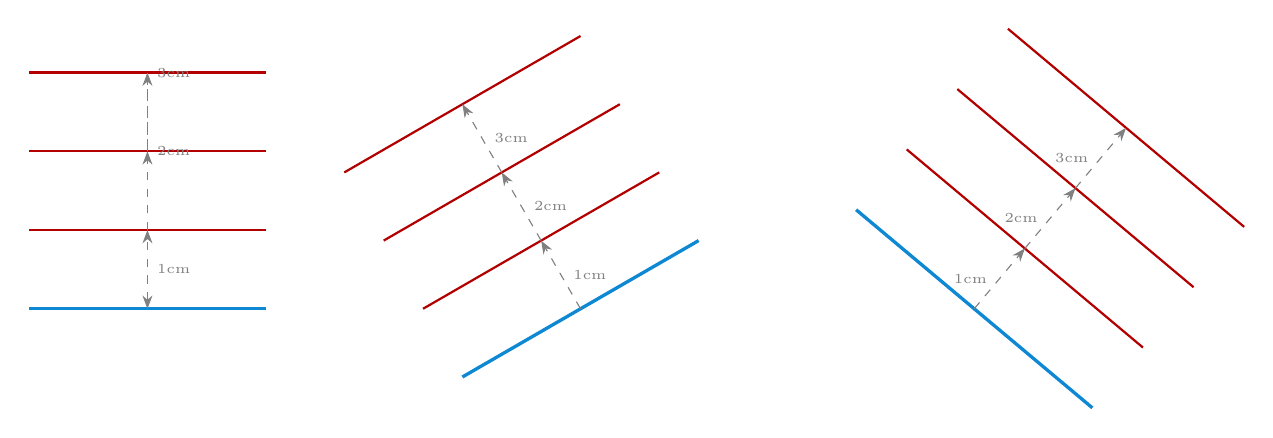
\begin{tikzpicture}[scale=1.0, >=Stealth]
    
    % 1. 水平线 (1, 2, 3 cm)
    \begin{scope}[xshift=0cm]
      % 已知直线 (y=0)
      \draw[cyan!70!blue, line width=1.2pt] (-1.5, 0) -- (1.5, 0);
      
      % 平行线 (上方)
      \draw[red!70!black, line width=0.8pt] (-1.5, 1) -- (1.5, 1);
      \draw[red!70!black, line width=0.8pt] (-1.5, 2) -- (1.5, 2);
      \draw[red!70!black, line width=0.8pt] (-1.5, 3) -- (1.5, 3);
      
      % 距离标注 (虚线箭头)
      \draw[gray, dashed, <->] (0, 0) -- (0, 1) node[midway, right, font=\tiny] {1cm};
      \draw[gray, dashed] (0, 1) -- (0, 3);
      \draw[gray, dashed, ->] (0, 1) -- (0, 2) node[pos=1, right, font=\tiny] {2cm};
      \draw[gray, dashed, ->] (0, 2) -- (0, 3) node[pos=1, right, font=\tiny] {3cm};
      
      %\node[below] at (0, -0.2) {场景 1: 水平线};
    \end{scope}

    % 2. 斜线 (中等斜率)，1, 2, 3 cm
    \begin{scope}[xshift=5.5cm]
      % 已知直线 (斜角 30度)
      \draw[cyan!70!blue, line width=1.2pt] (-1.5, -0.866) -- (1.5, 0.866);
      
      % 平行线 (垂直位移)
      % 法向角是 30 + 90 = 120 度
      \foreach \d in {1, 2, 3} {
        \draw[red!70!black, line width=0.8pt, shift={(120:\d)}] (-1.5, -0.866) -- (1.5, 0.866);
      }
      
      % 距离标注
      \draw[gray, dashed, ->] (0,0) -- (120:1) node[midway, right=1pt, font=\tiny] {1cm};
      \draw[gray, dashed, ->] (120:1) -- (120:2) node[midway, right=1pt, font=\tiny] {2cm};
      \draw[gray, dashed, ->] (120:2) -- (120:3) node[midway, right=1pt, font=\tiny] {3cm};

      %\node[below] at (0, -1.2) {场景 2: 斜线 (30$^\circ$)};
    \end{scope}

    % 3. 斜线 (较陡斜率)，1, 2, 3 cm
    \begin{scope}[xshift=10.5cm]
      % 已知直线 (斜角 -40度)
      \draw[cyan!70!blue, line width=1.2pt] (-1.5, 1.258) -- (1.5, -1.258);
      
      % 法向角是 -40 + 90 = 50 度
      \foreach \d in {1, 2, 3} {
        \draw[red!70!black, line width=0.8pt, shift={(50:\d)}] (-1.5, 1.258) -- (1.5, -1.258);
      }
      
      % 距离标注
      \draw[gray, dashed, ->] (0,0) -- (50:1) node[midway, left=1pt, font=\tiny] {1cm};
      \draw[gray, dashed, ->] (50:1) -- (50:2) node[midway, left=1pt, font=\tiny] {2cm};
      \draw[gray, dashed, ->] (50:2) -- (50:3) node[midway, left=1pt, font=\tiny] {3cm};

      %\node[below] at (0, -1.6) {场景 3: 斜线 (-40$^\circ$)};
    \end{scope}

  \end{tikzpicture}
\end{center}

\vspace{1.0cm}
\hrule
\vspace{0.4cm}

% 说明
{\small
\textbf{作图方法说明：} \\
1. \textbf{定垂线：} 在已知直线上找一点，画出已知直线的垂线。 \\
2. \textbf{取长度：} 在垂线上分别量出 1 厘米、2 厘米、3 厘米的长度，标出三个点。 \\
3. \textbf{画平行：} 过这三个点，分别画出已知直线的平行线。 \\
\textit{注：平行线也可以画在已知直线的另一侧，图中仅展示了一侧的画法。}
}


%% ==============================
%% 过点 A 画垂线和平行线，并量距离
%% ==============================
\newpage

\begin{center}
  {\large\bfseries 解答：过点 A 画垂线和平行线并量距离}
\end{center}

\vspace{0.6cm}

\noindent
{\small \textbf{题目要求：} 过点 A 分别画出已知直线的垂线和平行线，再量出点 A 到已知直线的距离。}

\vspace{0.8cm}

\begin{center}
  \begin{tikzpicture}[scale=1.2, >=Stealth]
    
    % 1. 点 A 在上方，斜线 (负斜率)
    \begin{scope}[xshift=0cm]
      % 已知直线 (斜率 -0.4)
      \draw[cyan!70!blue, line width=1.2pt] (-2, 0.8) -- (2, -0.8);
      
      % 点 A
      \node[vertex dot] (A1) at (0.5, 1.3) {};
      \node[right=4pt, font=\small] at (0.5, 1.3) {$A$};
      
      % 垂线 (斜率 2.5)
      % y - 1.3 = 2.5(x - 0.5) => y = 2.5x
      % 垂足计算: 0.4x + y = 0, y = 2.5x => 2.9x = 0 => x = 0, y = 0
      \draw[red!70!black, line width=1.0pt] (0.5, 1.3) -- (0, 0);
      \draw[red!70!black, line width=1.0pt, dashed] (0.5, 1.3) -- (0.7, 1.8);
      
      % 平行线 (斜率 -0.4)
      % y = -0.4x + 1.5
      \draw[red!70!black, line width=1.0pt] (-1.0, 1.9) -- (2.5, 0.5);
      
      % 直角符号 (旋转)
      % 直线角度: atan(-0.4) = -21.8 度
      \begin{scope}[shift={(0, 0)}, rotate=-21.8]
        \draw[red!70!black, thin] (0, 0.2) -- (0.2, 0.2) -- (0.2, 0);
      \end{scope}

      \node[below=2.5cm] at (0, 0) {(\quad 14\quad ) 毫米};
    \end{scope}

    % 2. 点 A 在下方，斜线 (正斜率)
    \begin{scope}[xshift=8cm]
      % 已知直线 (斜率 0.8)
      \draw[cyan!70!blue, line width=1.2pt] (-1.5, -1.2) -- (1.5, 1.2);
      
      % 点 A
      \node[vertex dot] (A2) at (1.5, -0.2) {};
      \node[right=4pt, font=\small] at (1.5, -0.2) {$A$};
      
      % 垂线 (斜率 -1.25)
      % y + 0.2 = -1.25(x - 1.5) => y = -1.25x + 1.675
      % 垂足计算: 0.8x = -1.25x + 1.675 => 2.05x = 1.675 => x = 0.817, y = 0.654
      \draw[red!70!black, line width=1.0pt] (1.5, -0.2) -- (0.817, 0.654);
      \draw[red!70!black, line width=1.0pt, dashed] (1.5, -0.2) -- (1.8, -0.575);
      
      % 平行线 (斜率 0.8)
      % y = 0.8x - 1.4
      \draw[red!70!black, line width=1.0pt] (0.0, -1.4) -- (2.5, 0.6);
      
      % 直角符号 (旋转)
      % 直线角度: atan(0.8) = 38.66 度
      \begin{scope}[shift={(0.817, 0.654)}, rotate=38.66]
        \draw[red!70!black, thin] (0, -0.2) -- (0.2, -0.2) -- (0.2, 0);
      \end{scope}

      \node[below=2.5cm] at (0.5, 0) {(\quad 11\quad ) 毫米};
    \end{scope}

  \end{tikzpicture}
\end{center}

\vspace{1.0cm}
\hrule
\vspace{0.4cm}

% 说明
{\small
\textbf{作图与测量说明：} \\
1. \textbf{画垂线：} 用三角尺的一条直角边与已知直线重合，另一条直角边经过点 A，沿边画出垂线，并标出直角符号。 \\
2. \textbf{画平行线：} 用三角尺的一条直角边与已知直线重合，另一条直角边靠紧直尺，平移三角尺使直角边经过点 A，画出平行线。 \\
3. \textbf{量距离：} 点 A 到已知直线的距离就是点 A 到垂足之间线段的长度。在尺子上量出该长度，单位转换为毫米。
}


%% ==============================
%% 画出从学校到公路的最短路线
%% ==============================
\newpage

\begin{center}
  {\large\bfseries 解答：画出从学校到公路的最短路线}
\end{center}

\vspace{0.6cm}

\noindent
{\small \textbf{题目要求：} 要修一条从学校到公路的小路，画出最短路线。}

\vspace{0.8cm}

\begin{center}
  \begin{tikzpicture}[scale=1.2, >=Stealth]
    
    % 公路 (双线折线) - 间距放大
    % 内缘: y=1.6, 折点 (1.25, 1.6), 坡度 -1
    % 外缘: y=2.4, 折点 (1.75, 2.4), 坡度 -1
    \draw[cyan!70!blue, line width=1.0pt] (-2.2, 2.4) -- (1.75, 2.4) -- (4.35, -0.2); % 外缘
    \draw[cyan!70!blue, line width=1.0pt] (-1.8, 1.6) -- (1.25, 1.6) -- (3.65, -0.8); % 内缘
    
    \node[above, cyan!80!blue] at (0, 2.4) {公路};
    \node[right, cyan!80!blue, rotate=-45] at (3.2, 0.2) {公路};
    
    % 学校 (点) - 坐标计算: (0.82, 0.4)
    % 距水平线 (y=1.6) 距离: 1.6 - 0.4 = 1.2cm = 12mm
    % 距斜线 (x+y=2.85) 距离: |0.82+0.4-2.85|/sqrt(2) = 1.63/1.414 = 1.152cm = 11.52mm
    \node[vertex dot, blue] (School) at (0.82, 0.4) {};
    \node[left=4pt, font=\small] at (0.82, 0.4) {学校};
    
    % 最短路线 (垂线，点到斜线最短)
    % 垂足计算: 
    % 斜线过 (1.25, 1.6), 斜率为 -1 => x+y = 2.85
    % 学校在 (0.82, 0.4), 垂线斜率为 1 => y-0.4 = x-0.82 => y = x - 0.42
    % 交点: x + (x - 0.42) = 2.85 => 2x = 3.27 => x = 1.635, y = 1.215
    \draw[red!70!black, line width=1.2pt] (0.82, 0.4) -- (1.635, 1.215);
    
    % 直角符号 (旋转并平移到垂足)
    \begin{scope}[shift={(1.635, 1.215)}, rotate=45]
      \draw[red!70!black, thin] (-0.2, 0) -- (-0.2, -0.2) -- (0, -0.2);
    \end{scope}
    
    \node[below=1.5cm] at (1, 0) {\textit{（最短路线为垂线段）}};
    
  \end{tikzpicture}
\end{center}

\vspace{1.0cm}
\hrule
\vspace{0.4cm}

% 说明
{\small
\textbf{原理说明：} \\
1. \textbf{点到直线的距离：} 直线外一点到这条直线的所有线段中，垂线段最短。 \\
2. \textbf{作图：} 从代表“学校”的点向代表“公路”的直线作垂线，这条垂线段就是从学校到公路的最短路线。
}


%% ==============================
%% 小鸭去小猫家怎样走比较省力
%% ==============================
\newpage

\begin{center}
  {\large\bfseries 解答：小鸭去小猫家怎样走比较省力}
\end{center}

\vspace{0.6cm}

\noindent
{\small \textbf{题目要求：} 小鸭在岸上走路比较吃力，却擅长游泳。它想到小猫家玩，从家出发，怎样走比较省力？}

\vspace{0.8cm}

\begin{center}
  \begin{tikzpicture}[scale=1.2, >=Stealth]
    
    % 小河 (不再平行的斜线)
    % 银行 1: x+y = 2 (斜率 -1)
    \draw[cyan!70!blue, line width=1.5pt] (-1, 3) -- (2, 0); 
    % 银行 2: 略微改变斜率，过 (0.5, 3.5) 和 (4, 0.5) (斜率 -0.857)
    \draw[cyan!70!blue, line width=1.5pt] (0.5, 3.5) -- (4, 0.5);
    
    \node[cyan!70!blue, font=\small] at (2.2, 0.8) {小河};
    
    % 家的位置
    \node[vertex dot, blue] (Duck) at (-1.5, 1.5) {};
    \node[left=4pt, font=\small] at (-1.5, 1.5) {小鸭家};
    
    \node[vertex dot, blue] (Cat) at (3.2, 2.5) {};
    \node[right=4pt, font=\small] at (3.2, 2.5) {小猫家};
    
    % 最省力路线 (红色垂线段 + 游泳)
    % 银行1: x+y = 2. 垂足 Foot1 为 (-0.5, 2.5)
    \draw[red!70!black, line width=1.2pt] (-1.5, 1.5) -- (-0.5, 2.5);
    
    % 银行2: 0.857*x + y = 3.9285. 垂足 Foot2 为 (2.55, 1.74)
    \draw[red!70!black, line width=1.2pt] (3.2, 2.5) -- (2.55, 1.74);
    
    % 游泳路线 (严格限制在河内)
    \draw[red!70!black, line width=1.2pt, dashed] (-0.5, 2.5) -- (2.55, 1.74);
    
    % 直角符号
    % 银行1 (斜率 -1, 旋转 -45)
    \begin{scope}[shift={(-0.5, 2.5)}, rotate=-45]
      \draw[red!70!black, thin] (0, -0.2) -- (0.2, -0.2) -- (0.2, 0);
    \end{scope}
    % 银行2 (斜率 -0.857, atan(-0.857) = -40.6 度)
    \begin{scope}[shift={(2.55, 1.74)}, rotate=-40.6]
      \draw[red!70!black, thin] (0, 0.2) -- (0.2, 0.2) -- (0.2, 0);
    \end{scope}
    
    \node[below=2cm] at (1, 0) {\textit{（省力路线：先垂直到岸边，再游泳，最后垂直去猫家）}};
    
  \end{tikzpicture}
\end{center}

\vspace{1.0cm}
\hrule
\vspace{0.4cm}

% 说明
{\small
\textbf{原理说明：} \\
1. \textbf{省力原则：} 因为小鸭在岸上走路吃力，所以应尽量缩短在岸上走的路程。 \\
2. \textbf{垂直最短：} 直线外一点到直线的所有线段中，垂线段最短。因此，从家向河岸作垂线，走路的路程最少。 \\
3. \textbf{作图步骤：} 分别从小鸭家和小猫家向对应的河岸作垂线，两段垂线段加上水中的游泳路线即为最省力路线。
}


%% ==============================
%% 长方形和正方形拼图
%% ==============================
\newpage

\begin{center}
  {\large\bfseries 解答：长方形和正方形拼图}
\end{center}

\vspace{0.6cm}

\noindent
{\small \textbf{题目要求：} 用一个长 6 厘米、宽 3 厘米的长方形和两个边长 3 厘米的正方形，可以拼成一个长方形，也可以拼成一个正方形。先在方格纸上画一画，再填空。}

\vspace{0.8cm}

\noindent
\textbf{1. 拼成长方形：} (可以拼成一个长 \textbf{12} 厘米、宽 \textbf{3} 厘米的长方形)

\begin{center}
  \begin{tikzpicture}[scale=0.5]
    % 网格
    \draw[cyan!30, thin] (0,0) grid (15, 5);
    
    % 拼成的长方形 (12 x 3)
    % 原始 6x3 长方形
    \fill[cyan!20] (1,1) rectangle (7,4);
    \draw[cyan!70!blue, thick] (1,1) rectangle (7,4);
    
    % 第一个 3x3 正方形
    \fill[red!20] (7,1) rectangle (10,4);
    \draw[red!70!black, thick] (7,1) rectangle (10,4);
    
    % 第二个 3x3 正方形
    \fill[yellow!20] (10,1) rectangle (13,4);
    \draw[yellow!70!black, thick] (10,1) rectangle (13,4);
    
    % 总外框 (不单独加外框，保持内部颜色区分)
    \node[below] at (7, 1) {\small 拼成长方形: $12 \times 3$};
  \end{tikzpicture}
\end{center}

\vspace{1.0cm}

\noindent
\textbf{2. 拼成正方形：} (可以拼成一个边长 \textbf{6} 厘米的正方形)

\begin{center}
  \begin{tikzpicture}[scale=0.5]
    % 网格
    \draw[cyan!30, thin] (0,0) grid (8, 8);
    
    % 拼成的正方形 (6 x 6)
    % 原始 6x3 长方形 (置于上方)
    \fill[cyan!20] (1,4) rectangle (7,7);
    \draw[cyan!70!blue, thick] (1,4) rectangle (7,7);
    
    % 第一个 3x3 正方形 (左下方)
    \fill[red!20] (1,1) rectangle (4,4);
    \draw[red!70!black, thick] (1,1) rectangle (4,4);
    
    % 第二个 3x3 正方形 (右下方)
    \fill[yellow!20] (4,1) rectangle (7,4);
    \draw[yellow!70!black, thick] (4,1) rectangle (7,4);
    
    \node[below] at (4, 1) {\small 拼成正方形: $6 \times 6$};
  \end{tikzpicture}
\end{center}

\vspace{1.0cm}
\hrule
\vspace{0.4cm}

% 说明
{\small
\textbf{解答填空：} \\
1. 可以拼成一个长 (\textbf{ 12 }) 厘米、宽 (\textbf{ 3 }) 厘米的长方形。 \\
2. 也可以拼成一个边长 (\textbf{ 6 }) 厘米的正方形。
}


%% ==============================
%% 利用直尺和圆规画图 (保留作图痕迹)
%% ==============================
\newpage

\begin{center}
  {\large\bfseries 解答：利用直尺和圆规画图 (保留作图痕迹)}
\end{center}

\vspace{0.6cm}

\begin{center}
  \begin{tikzpicture}[scale=0.8, >=Stealth]
    % (1) 画长 5cm, 宽 3cm 的长方形
    \begin{scope}[xshift=0cm]
      \coordinate (A) at (0,0);
      
      % 第一步: 画射线并作垂线
      \draw[cyan!70!blue, line width=1.0pt, ->] (-1,0) -- (6,0) node[right] {射线};
      \node[below left] at (A) {$A$};
      
      % 垂线痕迹 (以 A 为圆心截两点，再截上方)
      \draw[gray, thin] (0.8,0) arc (0:180:0.8);
      \coordinate (P1) at (-0.8,0);
      \coordinate (P2) at (0.8,0);
      \draw[gray, thin] (P1) ++(0.707, 0.707) arc (45:75:1);
      \draw[gray, thin] (P2) ++(-0.707, 0.707) arc (135:105:1);
      \draw[gray, dashed, thin] (0, -0.5) -- (0, 4) node[above] {垂线};
      
      % 第二步: 截取 B (5cm) 和 D (3cm)
      \draw[gray, thin] (5, 0.5) arc (90:45:0.7); % A 为圆心，R=5 截射线于 B
      \coordinate (B) at (5,0);
      \node[below] at (B) {$B$};
      
      \draw[gray, thin] (0.5, 3) arc (0:-35:0.7); % A 为圆心，R=3 截垂线于 D
      \coordinate (D) at (0,3);
      \node[left] at (D) {$D$};
      
      % 第三步: 以 B 为圆心 (R=3), D 为圆心 (R=5) 画弧相交于 C
      \draw[gray, thin] (D) ++(4.3, 0.3) arc (5:-5:5); % D 为圆心 R=5
      \draw[gray, thin] (B) ++(0.3, 2.3) arc (85:105:3); % B 为圆心 R=3 (修正: B 到 C 是宽，R=3)
      \coordinate (C) at (5,3);
      \node[above right] at (C) {$C$};
      
      % 第四步: 连接 BC, CD
      \draw[red!70!black, ultra thick] (A) -- (B) -- (C) -- (D) -- cycle;
      
      \node[below=1.2cm] at (2.5, 0) {\small (1) $5 \times 3$ 长方形};
    \end{scope}

    \begin{scope}[xshift=9cm]
      \coordinate (A) at (0,0);
      
      % 第一步: 画射线并作垂线
      \draw[cyan!70!blue, line width=1.0pt, ->] (-0.8,0) -- (3,0);
      \node[below left] at (A) {$A$};
      
      % 垂线痕迹
      \draw[gray, thin] (0.4,0) arc (0:180:0.4);
      \draw[gray, thin] (-0.4,0) ++(0.4, 0.6) arc (60:90:0.75);
      \draw[gray, thin] (0.4,0) ++(-0.4, 0.6) arc (120:90:0.75);
      \draw[gray, dashed, thin] (0, -0.5) -- (0, 3);
      
      % 第二步: 截取 B (2cm) 和 D (2cm)
      \draw[gray, thin] (2, 0.4) arc (90:30:0.5);
      \coordinate (B) at (2,0);
      \node[below] at (B) {$B$};
      
      \draw[gray, thin] (0.4, 2) arc (0:-30:0.5);
      \coordinate (D) at (0,2);
      \node[left] at (D) {$D$};
      
      % 第三步: 以 B, D 为圆心 (R=2) 画弧相交于 C
      \draw[gray, thin] (B) ++(0.3, 1.3) arc (80:110:2);
      \draw[gray, thin] (D) ++(1.3, 0.3) arc (10:-10:2);
      \coordinate (C) at (2,2);
      \node[above right] at (C) {$C$};
      
      % 第四步: 连接 BC, CD
      \draw[red!70!black, ultra thick] (A) -- (B) -- (C) -- (D) -- cycle;
      
      \node[below=1.2cm] at (1, 0) {\small (2) $2 \times 2$ 正方形};
    \end{scope}
  \end{tikzpicture}
\end{center}

\vspace{1.0cm}
\hrule
\vspace{0.4cm}

% 说明
{\small
\textbf{作图原理：} \\
1. \textbf{垂直：} 利用圆规在定线上截取等距两点，再以这两点为圆心，大于半径的一半为半径画弧，交点连线即为垂线。 \\
2. \textbf{度量：} 用圆规或直尺在垂线上量取指定高度，确定顶点。 \\
3. \textbf{封闭：} 连接各顶点，完成图形，并保留所有辅助圆弧痕迹。
}

\newpage

\section*{（1）画出长 5 厘米、宽 3 厘米的长方形}
\begin{center}
\begin{tikzpicture}[scale=1.2] % 稍微放大一点方便观察
    % 定义顶点坐标
    \coordinate (A) at (0,0);
    \coordinate (B) at (5,0);
    \coordinate (C) at (5,3);
    \coordinate (D) at (0,3);

    % 画基础射线和垂线（辅助线）
    \draw[-, thick, gray] (-1,0) -- (6.5,0) node[right] {\small 射线};
    \draw[-, thick, gray] (0,-1) -- (0,4.5) node[above] {\small 垂线};

    % === 精准保留作图痕迹（圆弧） ===
    % 1. 在射线上截取 AB = 5cm。圆心在 A(0,0)，半径为 5。
    % 弧线需要穿过 B(5,0)，且在 B 点与 X 轴垂直。
    % 我们让弧线关于 X 轴对称，角度范围设为 [-15, 15]。
    \draw[cyan, thick, dashed] ([shift=(-15:5)]A) arc [start angle=-15, end angle=15, radius=5];
    
    % 2. 在垂线上截取 AD = 3cm。圆心在 A(0,0)，半径为 3。
    % 弧线需要穿过 D(0,3)，且在 D 点与 Y 轴垂直。
    % 我们让弧线关于 Y 轴（90度）对称，角度范围设为 [75, 105]。
    \draw[cyan, thick, dashed] ([shift=(75:3)]A) arc [start angle=75, end angle=105, radius=3];

    % 3. 以 B(5,0) 为圆心，3cm 为半径在内部画弧。
    % 弧线需要穿过 C(5,3)，且在 C 点上方与 B 点保持垂直关系（即在 Y=3 处切线平）。
    % 目标点 C 在 B 点的 90 度方向（正上方）。
    % 我们让弧线关于 90 度对称，角度范围设为 [75, 105]。
    \draw[cyan, thick, dashed] ([shift=(75:3)]B) arc [start angle=75, end angle=105, radius=3];

    % 4. 以 D(0,3) 为圆心，5cm 为半径在内部画弧。
    % 弧线需要穿过 C(5,3)，且在 C 点右侧与 D 点保持水平关系（即在 X=5 处切线垂直）。
    % 目标点 C 在 D 点的 0 度方向（正右方）。
    % 我们让弧线关于 0 度（或360度）对称，角度范围设为 [-10, 10]。
    \draw[cyan, thick, dashed] ([shift=(-10:5)]D) arc [start angle=-10, end angle=10, radius=5];

    % === 连接长方形各边 ===
    \draw[thick] (A) -- (B) -- (C) -- (D) -- cycle;

    % 标注顶点字母
    \node[below left] at (A) {$A$};
    \node[below right] at (B) {$B$};
    \node[above right] at (C) {$C$};
    \node[above left] at (D) {$D$};
\end{tikzpicture}
\end{center}

\vspace{1cm}

\section*{（2）画出边长 2 厘米的正方形}
\begin{center}
\begin{tikzpicture}[scale=1.5] % 稍微放大一点
    % 定义顶点坐标
    \coordinate (A) at (0,0);
    \coordinate (B) at (2,0);
    \coordinate (C) at (2,2);
    \coordinate (D) at (0,2);

    % 画基础射线和垂线
    \draw[-, thick, gray] (-1,0) -- (3.5,0) node[right] {\small 射线};
    \draw[-, thick, gray] (0,-1) -- (0,3.5) node[above] {\small 垂线};

    % === 精准保留作图痕迹（圆弧） ===
    % 原理同上
    % 1. 截取 AB = 2cm (圆心A，半径2，穿过B(2,0))
    \draw[cyan, thick, dashed] ([shift=(-20:2)]A) arc [start angle=-20, end angle=20, radius=2];
    
    % 2. 截取 AD = 2cm (圆心A，半径2，穿过D(0,2))
    \draw[cyan, thick, dashed] ([shift=(70:2)]A) arc [start angle=70, end angle=110, radius=2];

    % 3. 以 B(2,0) 为圆心，2cm 为半径画弧穿过 C(2,2)
    % 目标点 C 在 B 点上方（90度），角度范围 [70, 110]。
    \draw[cyan, thick, dashed] ([shift=(70:2)]B) arc [start angle=70, end angle=110, radius=2];
    
    % 4. 以 D(0,2) 为圆心，2cm 为半径画弧穿过 C(2,2)
    % 目标点 C 在 D 点右方（0度），角度范围 [-20, 20]。
    \draw[cyan, thick, dashed] ([shift=(-20:2)]D) arc [start angle=-20, end angle=20, radius=2];

    % === 连接正方形各边 ===
    \draw[thick] (A) -- (B) -- (C) -- (D) -- cycle;

    % 标注顶点字母
    \node[below left] at (A) {$A$};
    \node[below right] at (B) {$B$};
    \node[above right] at (C) {$C$};
    \node[above left] at (D) {$D$};
\end{tikzpicture}
\end{center}



%% ==============================
%% 过直线外一点画垂线并画出正方形
%% ==============================
\newpage

\begin{center}
  {\large\bfseries 解答：过直线外一点画垂线并画出正方形}
\end{center}

\vspace{0.6cm}

\noindent
{\small \textbf{题目要求：} 先过直线外一点画已知直线的垂线，再沿着这一组垂线画出一个边长为 2 厘米的正方形。}

\vspace{1.0cm}

\begin{center}
  \begin{tikzpicture}[scale=1.2, >=Stealth]
    % 已知直线 (斜率 -0.4, 经过 (0,0))
    \draw[cyan!70!blue, line width=1.2pt] (-2, 0.8) -- (5, -2.0);
    \node[cyan!70!blue, right] at (5, -2.0) {\small 已知直线};
    
    % 已知点 A (距离直线恰好 1.7cm)
    % 垂线方向矢量 (1, 2.5). 单位矢量 (0.371, 0.928)
    % 距离 1.7cm => A = 1.7 * (0.371, 0.928) = (0.63, 1.58)
    \coordinate (A) at (0.63, 1.58);
    \node[vertex dot, blue] at (A) {};
    \node[left=4pt, blue, font=\small] at (A) {已知点 $A$};
    
    % 1. 过点 A 画垂线 (红色虚线)
    % 垂足 B 为 (0, 0). 延伸至 2.5cm 以覆盖正方形边长
    \draw[red!70!black, line width=0.8pt, dashed] (0, 0) -- (0.93, 2.32);
    
    % 直角符号
    \begin{scope}[rotate=-21.8]
      \draw[red!70!black, thin] (0, 0.2) -- (0.2, 0.2) -- (0.2, 0);
    \end{scope}
    
    % 2. 沿着垂线画边长为 2 厘米的正方形
    % 正方形顶点: B(0,0), D(0.74, 1.86) (沿垂线 2cm). D 在 A 之后 (1.86 > 1.58)
    % 另外两个顶点 C, E 沿直线方向平移 2cm
    % C = B + 2*(0.928, -0.371) = (1.86, -0.74)
    % E = D + 2*(0.928, -0.371) = (2.60, 1.12)
    \coordinate (B) at (0,0);
    \coordinate (C) at (1.86, -0.74);
    \coordinate (E) at (2.60, 1.12);
    \coordinate (D) at (0.74, 1.86);
    
    \draw[red!70!black, ultra thick] (B) -- (C) -- (E) -- (D) -- cycle;
    
    % 标注
    \node[below left, font=\small] at (B) {$B$};
    \node[below left, font=\small] at (C) {$C$};
    \node[above right, font=\small] at (E) {$E$};
    \node[right=4pt, font=\small] at (D) {$D$};

    % 距离标注 (1.7cm vs 2.0cm)
    %\draw[<->, gray, thin] (B) -- (A) node[midway, left, rotate=68.2] {\tiny 1.7 厘米};
    \node[red!70!black, rotate=-21.8, below] at (0.93, -0.37) {\small 2 厘米};
    %\node[red!70!black, rotate=68.2, right] at (2.2, 0.2) {\small 2 厘米};

  \end{tikzpicture}
\end{center}

\vspace{1.0cm}
\hrule
\vspace{0.4cm}

% 说明
{\small
\textbf{作图步骤：} \\
1. \textbf{画垂线：} 用三角尺的一条直角边与已知直线重合，另一条直角边经过点 $A$，沿直角边画线即为垂线。 \\
2. \textbf{定长度：} 在垂线上以点 $B$（垂足）为起点，截取 2 厘米得到点 $A$（已知点到直线的距离恰为 2 厘米）。 \\
3. \textbf{完成正方形：} 在已知直线上截取 $BC=2$ 厘米，过点 $C$ 作已知直线的垂线，截取 $CD=2$ 厘米，连接 $AD$（即为 $P$ 到 $D$）。
}


%% ==============================
%% 将正方形分割成大小正方形及等大长方形
%% ==============================
\newpage

\begin{center}
  {\large\bfseries 解答：将正方形分割成大小正方形及等大长方形}
\end{center}

\vspace{0.6cm}

\noindent
{\small \textbf{题目要求：} 在正方形中有一个点，过这个点可以将正方形分成一个小正方形、一个大正方形，以及两个大小相同的长方形，利用工具画出来。}

\vspace{1.0cm}

\begin{center}
  \begin{tikzpicture}[scale=1.5, >=Stealth]
    % 1. 原始正方形 (边长 4cm)
    \draw[cyan!70!blue, line width=1.2pt] (0, 0) rectangle (4, 4);
    
    % 2. 内部点 P (必须在对角线上以满足题目要求)
    % 选取坐标 (3, 3) 对应右上角的小区域
    \coordinate (P) at (3, 3);
    \node[vertex dot, blue] at (P) {};
    %\node[above right, blue, font=\small] at (P) {点 $P$};
    
    % 3. 画分割线
    % 水平线
    \draw[red!70!black, line width=1.0pt] (0, 3) -- (4, 3);
    % 铅垂线
    \draw[red!70!black, line width=1.0pt] (3, 0) -- (3, 4);
    
    % 4. 标注各个部分
    % 左下角：大正方形 (3x3)
    \node at (1.5, 1.5) {\small 大正方形};
    % 右上角：小正方形 (1x1)
    \node at (3.5, 3.5) {\small 小正方形};
    % 左上角：长方形 (3x1)
    \node at (1.5, 3.5) {\small 长方形};
    % 右下角：长方形 (1x3)
    \node at (3.5, 1.5) {\small 长方形};
    
    % 辅助标注：显示边长关系
    \draw[<->, gray, thin] (0, -0.3) -- (3, -0.3) node[midway, below] {\tiny $a$};
    \draw[<->, gray, thin] (3, -0.3) -- (4, -0.3) node[midway, below] {\tiny $b$};
    \draw[<->, gray, thin] (-0.3, 0) -- (-0.3, 3) node[midway, left] {\tiny $a$};
    \draw[<->, gray, thin] (-0.3, 3) -- (-0.3, 4) node[midway, left] {\tiny $b$};

  \end{tikzpicture}
\end{center}

\vspace{1.0cm}
\hrule
\vspace{0.4cm}

% 说明
{\small
\textbf{作图解析：} \\
1. \textbf{关键点判定：} 要将正方形分割成两个正方形和两个相等长方形，内部的点必须位于正方形的**对角线**上。 \\
2. \textbf{作图方法：} 确定对角线上的点 $P$ 后，分别画出经过点 $P$ 且平行于正方形各边的直线（水平线和铅垂线）。 \\
3. \textbf{分割结果：} 这样分割出的四个部分中，左下角和右上角必为正方形，左上角和右下角则为大小相同的长方形。
}


%% ==============================
%% 将正方形分割并拼成大三角形
%% ==============================
\newpage

\begin{center}
  {\large\bfseries 解答：将正方形分割并拼成大三角形}
\end{center}

\vspace{0.6cm}

\noindent
{\small \textbf{题目要求：} 一个正方形，沿着一条直线分成两部分，可以拼成一个大三角形。在图上先画出这条直线，再在右边画出拼成的大三角形。}

\vspace{1.0cm}

\begin{center}
  \begin{tikzpicture}[scale=1.2, >=Stealth]
    % 左侧图：正方形分割
    \begin{scope}[xshift=0cm]
      \draw[cyan!70!blue, line width=1.2pt] (0, 0) rectangle (3, 3);
      % 分割线 (对角线)
      \draw[red!70!black, line width=1.0pt, dashed] (0, 3) -- (3, 0);
      
      \node[below=0.5cm] at (1.5, 0) {\small (1) 沿对角线分割};
    \end{scope}
    
    % 箭头
    \draw[->, line width=1pt, gray] (4, 1.5) -- (5.5, 1.5) node[midway, above] {\tiny 重新拼接};
    
    % 右侧图：拼接后的大三角形
    \begin{scope}[xshift=8cm]
      % 拼接后的大三角形 (底边 6cm, 高 3cm)
      % 由两个 3x3x3*sqrt(2) 的等腰直角三角形拼成
      \coordinate (BottomLeft) at (-3, 0);
      \coordinate (BottomRight) at (3, 0);
      \coordinate (Top) at (0, 3);
      \coordinate (Mid) at (0, 0);
      
      \draw[cyan!70!blue, line width=1.2pt] (BottomLeft) -- (BottomRight) -- (Top) -- cycle;
      % 拼接缝
      \draw[red!70!black, line width=0.8pt, dashed] (Top) -- (Mid);
      
      \node[below=0.5cm] at (0, 0) {\small (2) 拼成的大三角形};
    \end{scope}

  \end{tikzpicture}
\end{center}

\vspace{1.0cm}
\hrule
\vspace{0.4cm}

% 说明
{\small
\textbf{作图解析：} \\
1. \textbf{分割方法：} 沿着正方形的一条**对角线**进行裁剪。 \\
2. \textbf{形状特征：} 裁剪后得到两个完全相同的**等腰直角三角形**。 \\
3. \textbf{拼接方法：} 将得到的两个等腰直角三角形的一条**直角边**完全重合，即可拼成一个较大的等腰三角形（其底边为原正方形边长的两倍，高为原正方形的边长）。
}


%% ==============================
%% 长方形连续剪正方形的过程
%% ==============================
\newpage

\begin{center}
  {\large\bfseries 解答：长方形连续剪正方形的过程}
\end{center}

\vspace{0.6cm}

\noindent
{\small \textbf{题目要求：} 一张长方形纸长 12 厘米、宽 7 厘米，先剪下一个最大的正方形，再从剩下的纸中剪下一个最大的正方形，最后剩下的图形是（\textbf{长方形}）。剩下图形的长和宽分别是（\textbf{5}）厘米与（\textbf{2}）厘米。}

\vspace{1.0cm}

\begin{center}
  \begin{tikzpicture}[scale=0.6, >=Stealth]
    % 1. 原始长方形轮廓 (12x7)
    \draw[cyan!70!blue, line width=1.2pt] (0, 0) rectangle (12, 7);
    
    % 2. 第一次剪裁：7x7 正方形 (从左侧开始)
    \draw[red!70!black, line width=1.0pt, dashed] (7, 0) -- (7, 7);
    \node at (3.5, 3.5) {\small 正方形①};
    \node at (3.5, 2.5) {\tiny $7\text{cm} \times 7\text{cm}$};
    
    % 3. 第二次剪裁：由 5x7 区域中剪出 5x5 正方形 (从底部开始)
    \draw[red!70!black, line width=1.0pt, dashed] (7, 5) -- (12, 5);
    \node at (9.5, 2.5) {\small 正方形②};
    \node at (9.5, 1.5) {\tiny $5\text{cm} \times 5\text{cm}$};
    
    % 4. 剩余区域 (5x2)
    \fill[red!10, opacity=0.5] (7, 5) rectangle (12, 7);
    \node at (9.5, 6) {\small\bfseries 剩余图形};
    \node at (9.5, 5.5) {\tiny $5\text{cm} \times 2\text{cm}$};
    
    % 5. 标注外围尺寸
    \draw[<->, gray, thin] (0, -0.8) -- (12, -0.8) node[midway, below] {\small 12 厘米};
    \draw[<->, gray, thin] (-0.8, 0) -- (-0.8, 7) node[midway, left, rotate=90] {\small 7 厘米};
    
    % 内部细分尺寸标注
    \draw[<->, gray, thin] (0, 7.5) -- (7, 7.5) node[midway, above] {\tiny 7};
    \draw[<->, gray, thin] (7, 7.5) -- (12, 7.5) node[midway, above] {\tiny 5};
    \draw[<->, gray, thin] (12.5, 0) -- (12.5, 5) node[midway, right] {\tiny 5};
    \draw[<->, gray, thin] (12.5, 5) -- (12.5, 7) node[midway, right] {\tiny 2};

  \end{tikzpicture}
\end{center}

\vspace{1.0cm}
\hrule
\vspace{0.4cm}

% 说明
{\small
\textbf{过程解析：} \\
1. \textbf{第一步：} 长 12 厘米、宽 7 厘米的长方形，最大的正方形边长为 7 厘米。 \\
   剪去后，剩下部分的长宽为：$12 - 7 = 5$（厘米），宽保持 $7$ 厘米。即得到一个 $5 \times 7$ 厘米的长方形。 \\
2. \textbf{第二步：} 在 $5 \times 7$ 厘米的长方形中，最大的正方形边长为 5 厘米。 \\
   剪去后，剩下部分的长宽为：$7 - 5 = 2$（厘米），另一边长保持 $5$ 厘米。 \\
3. \textbf{结论：} 最后剩下的图形是一个长为 **5 厘米**，宽为 **2 厘米** 的**长方形**。
}


%% ==============================
%% 纸张对折剪裁的对称性图形
%% ==============================
\newpage

\begin{center}
  {\large\bfseries 解答：纸张对折剪裁的对称性图形}
\end{center}

\vspace{0.6cm}

\noindent
{\small \textbf{题目要求：} 把正方形像图 1 这样对折两次，再画个圈并剪掉圈，打开后会是什么样？在图 2 中画一画。}

\vspace{1.0cm}

\begin{center}
  \begin{tikzpicture}[scale=1.2, >=Stealth]
    % --- 图 1：折叠过程 ---
    \begin{scope}[xshift=0cm, yshift=0cm]
      % 1. 初始
      \draw[cyan!70!blue, thin] (0,0) rectangle (2,2);
      \draw[->, gray] (2.2, 1) -- (2.8, 1);
      
      % 2. 第一次对折
      \begin{scope}[xshift=3cm]
        \draw[cyan!70!blue, thin] (1,0) rectangle (2,2);
        \draw[cyan!70!blue, dashed] (0,0) -- (1,0) -- (1,2) -- (0,2);
        \draw[->, blue, bend left] (0.5, 1.8) to node[above] {\tiny 翻折} (1.5, 1.8);
        \draw[->, gray] (2.2, 1) -- (2.8, 1);
      \end{scope}
      
      % 3. 第二次对折
      \begin{scope}[xshift=6cm]
        \draw[cyan!70!blue, thin] (1,0) rectangle (2,1);
        \draw[cyan!70!blue, dashed] (1,1) -- (1,2) -- (2,2) -- (2,1);
        \draw[->, blue, bend right] (1.2, 1.5) to node[left] {\tiny 翻折} (1.2, 0.5);
        \draw[->, gray] (2.2, 1) -- (2.8, 1);
      \end{scope}
      
      % 4. 最终裁剪
      \begin{scope}[xshift=9.5cm]
        \draw[cyan!70!blue, line width=1pt] (0,0) rectangle (1,1);
        \draw[red] (0.8, 0.8) circle (0.1);
        \node[below=0.2cm] at (0.5, 0) {\small 图 1：折叠与裁剪};
      \end{scope}
    \end{scope}

    % --- 图 2：解答 ---
    \begin{scope}[xshift=4.5cm, yshift=-7cm]
      \draw[cyan!70!blue, line width=1.2pt] (0,0) rectangle (4,4);
      % 折痕线
      \draw[cyan!70!blue, dashed, thin] (0,2) -- (4,2);
      \draw[cyan!70!blue, dashed, thin] (2,0) -- (2,4);
      
      

      % 4 个对称的圆孔
      % 原孔在右下象限的右上角 (此时原点 A 是左下)
      % 右下象限范围: [2,4] x [0,2]
      % 原孔位置: (3.6, 1.6)
      \draw[red, line width=1pt] (3.6, 1.6) circle (0.15);
      % 关于 y=2 对称 (上移)
      \draw[red, line width=1pt] (3.6, 2.4) circle (0.15);
      % 关于 x=2 对称 (左移)
      \draw[red, line width=1pt] (0.4, 1.6) circle (0.15);
      \draw[red, line width=1pt] (0.4, 2.4) circle (0.15);
      
      \node[below=0.5cm] at (2,0) {\large\bfseries 图 2：展开后的图案};
    \end{scope}
  \end{tikzpicture}
\end{center}

\vspace{1.0cm}
\hrule
\vspace{0.4cm}

% 说明
{\small
\textbf{原理分析：} \\
1. \textbf{对称轴：} 每次对折都会产生一条对称轴（折痕）。 \\
2. \textbf{镜像效应：} 剪掉一个圆孔后，展开过程相当于连续进行两次镜像反射。 \\
   - 第一次展开得到 2 个圆孔。 \\
   - 第二次展开得到 4 个圆孔。 \\
3. \textbf{分布规律：} 这 4 个圆孔关于水平中线和垂直中线严格对称，呈矩阵状分布在四个象限中。
}


%% ==============================
%% 火柴棒摆正方形趣题
%% ==============================
\newpage

\begin{center}
  {\large\bfseries 解答：火柴棒摆正方形趣题}
\end{center}

\vspace{0.6cm}

\noindent
{\small \textbf{题目要求：} 用 12 根火柴摆出 3 个正方形。小丽用 10 根火柴也正好摆了 3 个正方形，你能画出她摆的图形吗？}

\vspace{1.0cm}

\begin{center}
  \begin{tikzpicture}[scale=1.2, >=Stealth]
    % 自定义火柴样式: 粗线 + 红色/橙色圆头
    \tikzset{matchstick/.style={line width=2.5pt, gray!80, line cap=round}}
    \tikzset{matchhead/.style={fill=red!80!black}}

    % --- 左侧：12 根火柴 (原图参考) ---
    \begin{scope}[xshift=0cm]
      % 上方正方形 (4根)
      \draw[matchstick] (0.5, 1) -- (1.5, 1); \draw[matchstick] (0.5, 2) -- (1.5, 2);
      \draw[matchstick] (0.5, 1) -- (0.5, 2); \draw[matchstick] (1.5, 1) -- (1.5, 2);
      \fill[matchhead] (1.4, 1) circle (0.1); \fill[matchhead] (1.4, 2) circle (0.1);
      \fill[matchhead] (0.5, 1.9) circle (0.1); \fill[matchhead] (1.5, 1.9) circle (0.1);

      % 左下方正方形 (4根)
      \draw[matchstick] (-0.5, 0) -- (0.5, 0); \draw[matchstick] (-0.5, 1) -- (0.5, 1);
      \draw[matchstick] (-0.5, 0) -- (-0.5, 1); \draw[matchstick] (0.5, 0) -- (0.5, 1);
      \fill[matchhead] (0.4, 0) circle (0.1); \fill[matchhead] (0.4, 1) circle (0.1);
      \fill[matchhead] (-0.5, 0.9) circle (0.1); \fill[matchhead] (0.5, 0.9) circle (0.1);

      % 右下方正方形 (4根)
      \draw[matchstick] (1.5, 0) -- (2.5, 0); \draw[matchstick] (1.5, 1) -- (2.5, 1);
      \draw[matchstick] (1.5, 0) -- (1.5, 1); \draw[matchstick] (2.5, 0) -- (2.5, 1);
      \fill[matchhead] (2.4, 0) circle (0.1); \fill[matchhead] (2.4, 1) circle (0.1);
      \fill[matchhead] (1.5, 0.9) circle (0.1); \fill[matchhead] (2.5, 0.9) circle (0.1);

      \node[below=0.5cm] at (1, 0) {\small 12 根火柴（无共用边）};
    \end{scope}

    % 箭头
    \draw[->, line width=1pt, gray] (3.5, 1) -- (4.5, 1) node[midway, above] {\tiny 改进};

    % --- 右侧：10 根火柴 (小丽的摆法) ---
    \begin{scope}[xshift=6cm, yshift=0.5cm]
      % 三个横向排列的正方形 (共 10 根)
      % 水平线: 3根上 + 3根下 = 6根
      \foreach \x in {0,1,2} {
        \draw[matchstick] (\x, 0) -- (\x+1, 0);
        \draw[matchstick] (\x, 1) -- (\x+1, 1);
        \fill[matchhead] (\x+0.9, 0) circle (0.1);
        \fill[matchhead] (\x+0.9, 1) circle (0.1);
      }
      % 垂直线: 4根 (包含2根共用边) = 4根
      \foreach \x in {0,1,2,3} {
        \draw[matchstick] (\x, 0) -- (\x, 1);
        \fill[matchhead] (\x, 0.9) circle (0.1);
      }
      
      \node[below=1.0cm] at (1.5, 0) {\small 10 根火柴（共用边摆法）};
    \end{scope}

  \end{tikzpicture}
\end{center}

\vspace{1.0cm}
\hrule
\vspace{0.4cm}

% 说明
{\small
\textbf{解题思路：} \\
1. \textbf{火柴根数对比：} 摆一个独立的正方形需要 4 根火柴。3 个独立的正方形需要 $3 \times 4 = 12$ 根。 \\
2. \textbf{节省火柴的关键：} 让正方形之间**公用火柴棒**（共用边）。 \\
3. \textbf{摆法建议：} 将 3 个正方形横向（或纵向）排成一排。 \\
   - 内部的两条边被左右两边的正方形共同使用。 \\
   - 这样总共只需要：$4 (\text{第一个}) + 3 (\text{第二个}) + 3 (\text{第三个}) = 10$ 根火柴。
}


%% ==============================
%% 过点 A 画平行线和垂线
%% ==============================
\newpage

\begin{center}
  {\large\bfseries 解答：过点 A 画平行线和垂线}
\end{center}

\vspace{0.6cm}

\noindent
{\small \textbf{题目要求：} 过点 A 分别画出直线 $a$ 的平行线和直线 $b$ 的垂线。}

\vspace{1.0cm}

\begin{center}
  \begin{tikzpicture}[scale=1.2, >=Stealth]
    % 1. 定义背景直线 a 和 b
    % 交点 O (2, 1)
    \coordinate (O) at (2, 1);
    
    % 直线 a: 倾斜角约 30 度
    \draw[cyan!70!blue, line width=0.8pt] (0, 0) -- (4, 2) node[right, black] {$a$};
    
    % 直线 b: 倾斜角约 -20 度
    \draw[cyan!70!blue, line width=0.8pt] (0.5, 1.5) -- (4.5, 0.1) node[right, black] {$b$};
    
    % 2. 定义已知点 A
    \coordinate (A) at (3.5, 2.5);
    \node[vertex dot, blue] at (A) {};
    \node[right=3pt, blue] at (A) {$A$};
    
    % 3. 画解答部分 (红线)
    
    % 过 A 作 a 的平行线 (倾斜角同样为 30 度)
    % y - 2.5 = tan(30)*(x - 3.5)
    \draw[red!70!black, line width=1.2pt] (A) ++(210:3) -- (A) -- ++(30:2);
    \node[above left, red!70!black] at (3.5, 2.5) {\tiny 平行线};
    
    % 过 A 作 b 的垂线 (倾斜角 = -20 + 90 = 70 度)
    \draw[red!70!black, line width=1.2pt] (A) ++(250:2.5) -- (A) -- ++(70:0.5);
    \node[below right, red!70!black] at (3.5, 2.5) {\tiny 垂线};
    
    % 4. 标注直角符号
    % 垂线倾斜角 70, 直线 b 倾斜角 -20
    % 垂足位置大致在 (3.0, 0.6) 附近。为了精确，可以使用 TikZ 投影。
    \coordinate (Foot) at ($(0.5, 1.5)!(A)!(4.5, 0.1)$);
    \draw[red!70!black, thin] (Foot) -- ++(70:0.3) -- ++(-20:0.3) -- ++(250:0.3);

  \end{tikzpicture}
\end{center}

\vspace{1.0cm}
\hrule
\vspace{0.4cm}

% 说明
{\small
\textbf{作图步骤：} \\
1. \textbf{画平行线：} 将三角尺的一条直角边与直线 $a$ 重合，用直尺紧靠三角尺的另一条直角边；沿直尺推动三角尺，使原直角边经过点 $A$，沿该边画出直线，即为直线 $a$ 的平行线。 \\
2. \textbf{画垂线：} 将三角尺的一条直角边与直线 $b$ 重合；沿直线 $b$ 移动三角尺，使三角尺的另一条直角边经过点 $A$，沿该边画出直线，即为直线 $b$ 的垂线。标出直角符号。
}


%% ==============================
%% 小河过河最短路线
%% ==============================
\newpage

\begin{center}
  {\large\bfseries 解答：小河过河最短路线}
\end{center}

\vspace{0.6cm}

\noindent
{\small \textbf{题目要求：} 如图，一艘汽艇由点 $A$ 开到河对岸，怎样开路线最短？把路线画出来。}

\vspace{1.0cm}

\begin{center}
  \begin{tikzpicture}[scale=1.5, >=Stealth]
    % 1. 绘制河岸
    % 下岸 (水平)
    \draw[cyan!70!blue, line width=1.0pt] (0, 0) -- (6, 0);
    % 上岸 (倾斜)
    \draw[cyan!70!blue, line width=1.0pt] (0, 1) -- (5.5, 2.5);
    \node[right] at (6, 1.2) {\small 小河};
    
    % 2. 绘制水纹效果 (装饰性)
    \foreach \n in {1,2,...,15}{
      \draw[cyan!40!white, thin] ({rand*2.5+3}, {rand*0.6+0.8}) -- ++(0.3, 0);
    }
    
    % 3. 定义出发点 A
    \coordinate (A) at (2.5, 0);
    \node[vertex dot, blue] at (A) {};
    \node[below, blue] at (A) {$A$};
    
    % 4. 计算并绘制最短路线 (垂线段)
    % 对岸直线经过 (0, 1) 和 (5.5, 2.5)
    % 向量 D = (5.5, 1.5)
    % 点 P0 = (0, 1)
    \coordinate (BankTopStart) at (0, 1);
    \coordinate (BankTopEnd) at (5.5, 2.5);
    
    % 使用 TikZ 投影
    \coordinate (Foot) at ($(BankTopStart)!(A)!(BankTopEnd)$);
    
    % 绘制红色的最短路线
    \draw[red!70!black, line width=1.5pt, dashed] (A) -- (Foot);
    \node[right=3pt, red!70!black, font=\tiny, rotate=15.25] at ($(A)!0.5!(Foot)$) {最短路线};
    
    % 5. 标注直角符号
    % 上岸倾斜角 atan(1.5/5.5) 约为 15.25 度
    % 垂线倾斜角约为 105.25 度
    \draw[red!70!black, thin] (Foot) -- ++(285.25:0.25) -- ++(15.25:0.25) -- ++(105.25:0.25);

  \end{tikzpicture}
\end{center}

\vspace{1.0cm}
\hrule
\vspace{0.4cm}

% 说明
{\small
\textbf{作图解析：} \\
1. \textbf{核心原理：} 从直线外一点到这条直线所画的所有线段中，**垂直线段**最短。 \\
2. \textbf{作图方法：} 利用三角尺的直角边，将其一条边与河对岸的直线重合，另一条边经过点 $A$，画出点 $A$ 到对岸的垂直线段。 \\
3. \textbf{结论：} 这条垂直线段即为汽艇行驶的最短路线。在对岸交点处应标出直角符号。
}


%% ==============================
%% 将正方形平均分成 4 份的四种方法
%% ==============================
\newpage

\begin{center}
  {\large\bfseries 解答：将正方形平均分成 4 份的四种方法}
\end{center}

\vspace{0.6cm}

\noindent
{\small \textbf{题目要求：} 把正方形平均分成完全相同的 4 份，你有几种不同的方法？在下图中心画一画。}

\vspace{1.0cm}

\begin{center}
  \begin{tikzpicture}[scale=1.0, >=Stealth]
    % 定义基础距离
    \def\sqsize{2.5}
    \def\spacing{3.5}

    % --- 方法 1：中位线法 (田字) ---
    \begin{scope}[xshift=0*\spacing cm]
      \draw[cyan!70!blue, line width=1pt] (0,0) rectangle (\sqsize, \sqsize);
      \draw[red!70!black, line width=1pt] (0.5*\sqsize, 0) -- (0.5*\sqsize, \sqsize);
      \draw[red!70!black, line width=1pt] (0, 0.5*\sqsize) -- (\sqsize, 0.5*\sqsize);
      \node[below=0.3cm] at (0.5*\sqsize, 0) {\small ① 中位线法};
    \end{scope}

    % --- 方法 2：竖向条状 ---
    \begin{scope}[xshift=1*\spacing cm]
      \draw[cyan!70!blue, line width=1pt] (0,0) rectangle (\sqsize, \sqsize);
      \foreach \i in {1,2,3}{
        \draw[red!70!black, line width=1pt] (\i/4*\sqsize, 0) -- (\i/4*\sqsize, \sqsize);
      }
      \node[below=0.3cm] at (0.5*\sqsize, 0) {\small ② 竖向条状};
    \end{scope}

    % --- 方法 3：横向条状 ---
    \begin{scope}[xshift=2*\spacing cm]
      \draw[cyan!70!blue, line width=1pt] (0,0) rectangle (\sqsize, \sqsize);
      \foreach \i in {1,2,3}{
        \draw[red!70!black, line width=1pt] (0, \i/4*\sqsize) -- (\sqsize, \i/4*\sqsize);
      }
      \node[below=0.3cm] at (0.5*\sqsize, 0) {\small ③ 横向条状};
    \end{scope}

    % --- 方法 4：对角线法 ---
    \begin{scope}[xshift=3*\spacing cm]
      \draw[cyan!70!blue, line width=1pt] (0,0) rectangle (\sqsize, \sqsize);
      \draw[red!70!black, line width=1pt] (0,0) -- (\sqsize, \sqsize);
      \draw[red!70!black, line width=1pt] (0, \sqsize) -- (\sqsize, 0);
      \node[below=0.3cm] at (0.5*\sqsize, 0) {\small ④ 对角线法};
    \end{scope}

  \end{tikzpicture}
\end{center}

\vspace{1.0cm}
\hrule
\vspace{0.4cm}

% 说明
{\small
\textbf{解题思路：} \\
1. \textbf{基本要求：} “平均分”意味着面积相等，“完全相同”意味着形状全等。 \\
2. \textbf{主要方法：} \\
   - **中位线法**：连接对边的中点，形成 4 个全等的小正方形。 \\
   - **条状分法**：将一组对边 4 等分，连结对应点，形成 4 个全等的长方形（可横分或竖分）。 \\
   - **对角线法**：连接两条对角线，形成 4 个全等的等腰直角三角形。 \\
3. \textbf{知识拓展：} 除了这四种最基础的方法外，还可以通过过中心的任意两条互相垂直的直线进行无限种分割，只要保证旋转对称性。
}


%% ==============================
%% 利用 12 个小正方形拼长方形
%% ==============================
\newpage

\begin{center}
  {\large\bfseries 解答：利用 12 个小正方形拼长方形}
\end{center}

\vspace{0.6cm}

\noindent
{\small \textbf{题目要求：} 有 12 个边长为 1 厘米的正方形，可以拼成几种不同的长方形？画一画。}

\vspace{1.0cm}

\begin{center}
  \begin{tikzpicture}[scale=0.6, >=Stealth]
    % 定义比例：1个单位代表 1cm，缩放 0.6 倍以便排版
    \def\spacing{3.0}

    % --- 方案 1：1 x 12 ---
    \begin{scope}[yshift=4cm]
      \draw[cyan!70!blue, line width=1pt] (0,0) rectangle (12, 1);
      \foreach \i in {1,...,11}{
        \draw[gray!40, thin] (\i, 0) -- (\i, 1);
      }
      \node[below=0.2cm] at (6, 0) {\small ① 长 12 \text{cm}，宽 1 \text{cm}};
    \end{scope}

    % --- 方案 2：2 x 6 ---
    \begin{scope}[yshift=-1cm]
      \draw[cyan!70!blue, line width=1pt] (0,0) rectangle (6, 2);
      \draw[gray!40, thin] (0, 1) -- (6, 1); % 横向中线
      \foreach \i in {1,...,5}{
        \draw[gray!40, thin] (\i, 0) -- (\i, 2);
      }
      \node[below=0.2cm] at (3, 0) {\small ② 长 6 \text{cm}，宽 2 \text{cm}};
    \end{scope}

    % --- 方案 3：3 x 4 ---
    \begin{scope}[xshift=8cm, yshift=-1cm]
      \draw[cyan!70!blue, line width=1pt] (0,0) rectangle (4, 3);
      \foreach \j in {1,2}{
        \draw[gray!40, thin] (0, \j) -- (4, \j);
      }
      \foreach \i in {1,2,3}{
        \draw[gray!40, thin] (\i, 0) -- (\i, 3);
      }
      \node[below=0.2cm] at (2, 0) {\small ③ 长 4 \text{cm}，宽 3 \text{cm}};
    \end{scope}

  \end{tikzpicture}
\end{center}

\vspace{1.0cm}
\hrule
\vspace{0.4cm}

% 说明
{\small
\textbf{解题思路：} \\
1. \textbf{核心原理：} 拼成的长方形面积必须等于 12 个小正方形的面积之和，即 $12 \times 1 = 12$ 平方厘米。 \\
2. \textbf{寻找因数对：} 通过寻找 12 的正整数因子对 $(a, b)$，即可确定长方形的长和宽。 \\
   - $12 = 1 \times 12$ \\
   - $12 = 2 \times 6$ \\
   - $12 = 3 \times 4$ \\
3. \textbf{结论：} 共有 **3 种** 不同的拼法（注：在小学数学中，$1 \times 12$ 与 $12 \times 1$ 被视为同一种形状的不同摆放方式，故计为 1 种）。
}


%% ==============================
%% 在平行线间画长是宽 2 倍的长方形
%% ==============================
\newpage

\begin{center}
  {\large\bfseries 解答：在平行线间画长是宽 2 倍的长方形}
\end{center}

\vspace{0.6cm}

\noindent
{\small \textbf{题目要求：} 从下面的两条平行线中取一段长度作为长方形的一组对边，画出一个长是宽的 2 倍的长方形。你能画出不同的长方形吗？}

\vspace{1.0cm}

\begin{center}
  \begin{tikzpicture}[scale=1.2, >=Stealth]
    % 定义比例：距离 d = 1.5 cm
    \def\dist{1.5}
    \def\Lwide{3.0}     % 2 * 1.5
    \def\Wnarrow{0.75}  % 1.5 / 2

    % --- 绘制背景平行线 ---
    \draw[cyan!70!blue, line width=0.8pt] (-1, \dist) -- (9, \dist);
    \draw[cyan!70!blue, line width=0.8pt] (-1, 0) -- (9, 0);

    % --- 方案 A：间距 d 为宽 (W=d)，则 长 L = 2d = 3.0 ---
    \begin{scope}[xshift=0.5cm]
      \draw[red!70!black, line width=1.2pt] (0, 0) rectangle (\Lwide, \dist);
      \node[below, red!70!black] at (0.5*\Lwide, 0) {\tiny 长};
      \node[right, red!70!black] at (\Lwide, 0.5*\dist) {\tiny 宽};
      \node[above=0.8cm] at (0.5*\Lwide, \dist) {\small ① “横向”长方形};
    \end{scope}

    % --- 方案 B：间距 d 为长 (L=d)，则 宽 W = d/2 = 0.75 ---
    \begin{scope}[xshift=6.5cm]
      \draw[red!70!black, line width=1.2pt] (0, 0) rectangle (\Wnarrow, \dist);
      \node[below, red!70!black] at (0.5*\Wnarrow, 0) {\tiny 宽};
      \node[right, red!70!black] at (\Wnarrow, 0.5*\dist) {\tiny 长};
      \node[above=0.8cm] at (0.5*\Wnarrow, \dist) {\small ② “纵向”长方形};
    \end{scope}

  \end{tikzpicture}
\end{center}

\vspace{1.0cm}
\hrule
\vspace{0.4cm}

% 说明
{\small
\textbf{作图解析：} \\
1. \textbf{核心原理：} 长方形的一组对边在平行线上，说明其“高度”固定为两条平行线间的垂直距离 $d$。 \\
2. \textbf{方案讨论：} 根据“长是宽的 2 倍” ($L = 2W$)，有两种不同的对应方式： \\
   - **情况 ①**：将间距 $d$ 作为**宽** ($W=d$)，则在平行线上的边长应为**长** ($L=2d$)。 \\
   - **情况 ②**：将间距 $d$ 作为**长** ($L=d$)，则在平行线上的边长应为**宽** ($W=d/2$)。 \\
3. \textbf{结论：} 可以画出不同的长方形，它们的比例关系相同，但相对于平行线的朝向和具体尺寸不同。
}


%% ==============================
%% 在正方形中表示分数 (1/2, 1/4, 1/8)
%% ==============================
\newpage

\begin{center}
  {\large\bfseries 解答：在正方形中表示分数}
\end{center}

\vspace{0.6cm}

\noindent
{\small \textbf{题目要求：} 下面是一张正方形纸，你能表示出它的 $\frac{1}{2}$, $\frac{1}{4}$, $\frac{1}{8}$ 吗？画一画。}

\vspace{1.0cm}

\begin{center}
  \begin{tikzpicture}[scale=1.2, >=Stealth]
    % 定义基础正方形边长
    \def\sqs{2.5}
    \def\gap{4.0}

    % --- 方案 1：表示 1/2 ---
    \begin{scope}[xshift=0*\gap cm]
      % 填充 1/2
      \fill[cyan!20] (0, 0) rectangle (0.5*\sqs, \sqs);
      % 画边框和分割线
      \draw[cyan!70!blue, line width=1pt] (0, 0) rectangle (\sqs, \sqs);
      \draw[black!60, thin] (0.5*\sqs, 0) -- (0.5*\sqs, \sqs);
      \node[below=0.4cm] at (0.5*\sqs, 0) {\large $\frac{1}{2}$};
    \end{scope}

    % --- 方案 2：表示 1/4 ---
    \begin{scope}[xshift=1*\gap cm]
      % 填充 1/4 (左上角)
      \fill[cyan!20] (0, 0.5*\sqs) rectangle (0.5*\sqs, \sqs);
      % 画边框和分割线
      \draw[cyan!70!blue, line width=1pt] (0, 0) rectangle (\sqs, \sqs);
      \draw[black!60, thin] (0.5*\sqs, 0) -- (0.5*\sqs, \sqs);
      \draw[black!60, thin] (0, 0.5*\sqs) -- (\sqs, 0.5*\sqs);
      \node[below=0.4cm] at (0.5*\sqs, 0) {\large $\frac{1}{4}$};
    \end{scope}

    % --- 方案 3：表示 1/8 ---
    \begin{scope}[xshift=2*\gap cm]
      % 填充 1/8 (左上角四个三角形中的一个)
      \fill[cyan!20] (0, \sqs) -- (0.5*\sqs, 0.5*\sqs) -- (0, 0.5*\sqs) -- cycle;
      % 画边框和分割线
      \draw[cyan!70!blue, line width=1pt] (0, 0) rectangle (\sqs, \sqs);
      \draw[black!60, thin] (0.5*\sqs, 0) -- (0.5*\sqs, \sqs);
      \draw[black!60, thin] (0, 0.5*\sqs) -- (\sqs, 0.5*\sqs);
      \draw[black!60, thin] (0, 0) -- (\sqs, \sqs);
      \draw[black!60, thin] (0, \sqs) -- (\sqs, 0);
      \node[below=0.4cm] at (0.5*\sqs, 0) {\large $\frac{1}{8}$};
    \end{scope}

  \end{tikzpicture}
\end{center}

\vspace{1.0cm}
\hrule
\vspace{0.4cm}

% 说明
{\small
\textbf{解题思路：} \\
1. \textbf{表示 $\frac{1}{2}$}：将正方形对折一次，分成两个完全相同的长方形，涂色其中一份即可。 \\
2. \textbf{表示 $\frac{1}{4}$}：将正方形横竖各对折一次，分成四个完全相同的小正方形，涂色其中一份即可。 \\
3. \textbf{表示 $\frac{1}{8}$}：在分成四份的基础上，再沿着每个小格子的对角线对折，分成八个完全相同的等腰直角三角形，涂色其中一份即可。 \\
*(注：分割方法不唯一，只要保证每一份面积相等且总量为对应的分数即可。)*
}


%% ==============================
%% 分数的涂色与小数表示 (2/10, 5/10, 9/10)
%% ==============================
\newpage

\begin{center}
  {\large\bfseries 解答：分数的涂色与小数表示}
\end{center}

\vspace{0.6cm}

\noindent
{\small \textbf{题目要求：} 先涂色表示分数，再用小数表示。}

\vspace{1.0cm}

\begin{center}
  \begin{tikzpicture}[scale=1.2, >=Stealth]
    % 定义基础正方形参数
    \def\sqs{2.5}
    \def\gap{5.2}

    % --- 方案 1：2/10 ---
    \begin{scope}[xshift=0*\gap cm]
      % 填充 2/10
      \fill[cyan!20] (0, 0) rectangle (0.2*\sqs, \sqs);
      % 画边框和 10 条竖线
      \draw[cyan!70!blue, line width=1pt] (0, 0) rectangle (\sqs, \sqs);
      \foreach \i in {1,...,9}{
        \draw[cyan!70!blue, dashed, thin] (\i/10*\sqs, 0) -- (\i/10*\sqs, \sqs);
      }
      % 标注分数和小数
      \node[right=0.8cm] at (\sqs, 0.6*\sqs) {\large $\frac{2}{10}$};
      \node[right=0.8cm] at (\sqs, 0.2*\sqs) {\large $(\quad 0.2 \quad)$};
    \end{scope}

    % --- 方案 2：5/10 ---
    \begin{scope}[xshift=1*\gap cm]
      % 填充 5/10
      \fill[cyan!20] (0, 0) rectangle (0.5*\sqs, \sqs);
      % 画边框和 10 条竖线
      \draw[cyan!70!blue, line width=1pt] (0, 0) rectangle (\sqs, \sqs);
      \foreach \i in {1,...,9}{
        \draw[cyan!70!blue, dashed, thin] (\i/10*\sqs, 0) -- (\i/10*\sqs, \sqs);
      }
      % 标注分数和小数
      \node[right=0.8cm] at (\sqs, 0.6*\sqs) {\large $\frac{5}{10}$};
      \node[right=0.8cm] at (\sqs, 0.2*\sqs) {\large $(\quad 0.5 \quad)$};
    \end{scope}

    % --- 方案 3：9/10 ---
    \begin{scope}[xshift=2*\gap cm]
      % 填充 9/10
      \fill[cyan!20] (0, 0) rectangle (0.9*\sqs, \sqs);
      % 画边框和 10 条竖线
      \draw[cyan!70!blue, line width=1pt] (0, 0) rectangle (\sqs, \sqs);
      \foreach \i in {1,...,9}{
        \draw[cyan!70!blue, dashed, thin] (\i/10*\sqs, 0) -- (\i/10*\sqs, \sqs);
      }
      % 标注分数和小数
      \node[right=0.8cm] at (\sqs, 0.6*\sqs) {\large $\frac{9}{10}$};
      \node[right=0.8cm] at (\sqs, 0.2*\sqs) {\large $(\quad 0.9 \quad)$};
    \end{scope}

  \end{tikzpicture}
\end{center}

\vspace{1.0cm}
\hrule
\vspace{0.4cm}

% 说明
{\small
\textbf{知识要点：} \\
1. \textbf{十分之几与一位小数}：分母是 10 的分数可以用一位小数来表示。 \\
2. \textbf{对应关系}： \\
   - $\frac{2}{10}$ 表示把一个整体平均分成 10 份，取其中的 2 份，写成小数是 $0.2$。 \\
   - $\frac{5}{10}$ 表示把一个整体平均分成 10 份，取其中的 5 份（即一半），写成小数是 $0.5$。 \\
   - $\frac{9}{10}$ 表示把一个整体平均分成 10 份，取其中的 9 份，写成小数是 $0.9$。
}


%% ==============================
%% 比较 1/3 和 1/4 的大小
%% ==============================
\newpage

\begin{center}
  {\large\bfseries Gemini 3 flash(antigravity)解答：为什么 $\frac{1}{3} > \frac{1}{4}$}
\end{center}

\vspace{0.6cm}

\noindent
{\small \textbf{题目要求：} 画图或写文字说明：为什么 $\frac{1}{3} > \frac{1}{4}$？}

\vspace{1.0cm}

\begin{center}
  \begin{tikzpicture}[scale=1.2, >=Stealth]
    % 定义长方形总宽和高
    \def\totalW{6}
    \def\rectH{1.2}

    % --- 图甲：表示 1/3 ---
    \begin{scope}[yshift=2.5cm]
      % 填充 1/3
      \fill[cyan!20] (0, 0) rectangle (1/3*\totalW, \rectH);
      % 画边框和分割线
      \draw[cyan!70!blue, line width=1pt] (0, 0) rectangle (\totalW, \rectH);
      \foreach \i in {1,2}{
        \draw[cyan!70!blue, thin] (\i/3*\totalW, 0) -- (\i/3*\totalW, \rectH);
      }
      \node[left=0.3cm] at (0, 0.5*\rectH) {\large $\frac{1}{3}$};
      \node[below=0.1cm] at (1/6*\totalW, 0) {\tiny 已涂 1 份};
    \end{scope}

    % --- 图乙：表示 1/4 ---
    \begin{scope}[yshift=0cm]
      % 填充 1/4
      \fill[cyan!20] (0, 0) rectangle (1/4*\totalW, \rectH);
      % 画边框和分割线
      \draw[cyan!70!blue, line width=1pt] (0, 0) rectangle (\totalW, \rectH);
      \foreach \i in {1,2,3}{
        \draw[cyan!70!blue, thin] (\i/4*\totalW, 0) -- (\i/4*\totalW, \rectH);
      }
      \node[left=0.3cm] at (0, 0.5*\rectH) {\large $\frac{1}{4}$};
      \node[below=0.1cm] at (1/8*\totalW, 0) {\tiny 已涂 1 份};
    \end{scope}

    % --- 辅助对比线 ---
    \draw[red, dashed, line width=0.8pt] (1/4*\totalW, -0.5) -- (1/4*\totalW, 4.0);
    \draw[red, dashed, line width=0.8pt] (1/3*\totalW, -0.5) -- (1/3*\totalW, 4.0);
    \node[red, above] at (1/3*\totalW, 4.0) {\tiny 1/3 的边界};
    \node[red, below] at (1/4*\totalW, -0.5) {\tiny 1/4 的边界};

  \end{tikzpicture}
\end{center}

\vspace{1.0cm}
\hrule
\vspace{0.4cm}

% 说明
{\small
\textbf{结论与解析：} \\
1. \textbf{直观对比}：从图中可以看出，同样的两个长方形（整体 1 相同），平均分成 3 份后其中的 1 份，比平均分成 4 份后其中的 1 份面积要**大**。 \\
2. \textbf{逻辑推导}：
   - 因为两个相同的整体，平均分的份数越多，每一份就越小。
   - $3 < 4$，说明分成的份数较少。
   - 所以，$\frac{1}{3}$ 得到的那一份比 $\frac{1}{4}$ 得到的那一份要大。
3. \textbf{数学规律}：分子相同的两个分数，分母小的分数比较大。
}

\section*{gpt-5.2-codex}

\begin{tikzpicture}[scale=1]
% 第一条：1/3
\draw (0,0) rectangle (6,1);
\foreach \x in {2,4} {
  \draw (\x,0) -- (\x,1);
}
\fill[gray!40] (0,0) rectangle (2,1);
\node at (3,-0.4) {$\dfrac{1}{3}$};
% 第二条：1/4
\draw (0,-2) rectangle (6,-1);
\foreach \x in {1.5,3,4.5} {
  \draw (\x,-2) -- (\x,-1);
}
\fill[gray!40] (0,-2) rectangle (1.5,-1);
\node at (3,-2.4) {$\dfrac{1}{4}$};
% 大于号
\node at (7, -1) {\Large $>$};
\end{tikzpicture}

\section*{gpt-5.4}

\begin{tikzpicture}[scale=1]
% 上面：1/3
\draw (0,2) rectangle (9,3);
\draw (3,2) -- (3,3);
\draw (6,2) -- (6,3);
\fill[blue!30] (0,2) rectangle (3,3);
\node[left] at (0,2.5) {$\frac{1}{3}$};
% 下面：1/4
\draw (0,0) rectangle (9,1);
\draw (2.25,0) -- (2.25,1);
\draw (4.5,0) -- (4.5,1);
\draw (6.75,0) -- (6.75,1);
\fill[red!30] (0,0) rectangle (2.25,1);
\node[left] at (0,0.5) {$\frac{1}{4}$};
% 说明文字
\node at (4.5,-0.8) {同样大的整体，平均分成的份数越多，每一份越小。};
\node at (4.5,-1.5) {所以 $\frac{1}{3}>\frac{1}{4}$。};
\end{tikzpicture}


%% ==============================
%% 黑板报版面比例问题 (1/3, 1/3, 1/6, 1/6)
%% ==============================
\newpage

\begin{center}
  {\large\bfseries 解答：黑板报版面比例问题}
\end{center}

\vspace{0.6cm}

\noindent
{\small \textbf{题目要求：} 新学期三(2)班的黑板报一共设置了四个栏目。其中，“知识窗”占黑板报的 $\frac{1}{3}$，剩下的 $\frac{1}{2}$ 为“科学园地”，“安全角”和“新学期寄语”各占了最后剩下的一半。“安全角”和“新学期寄语”各占黑板报的几分之几？（先在图中画一画，再回答。）}

\vspace{1.0cm}

\begin{center}
  \begin{tikzpicture}[scale=1.5, >=Stealth]
    % 定义黑板总尺寸
    \def\totalW{6}
    \def\totalH{4}

    % --- 绘制各区域并填充颜色 ---
    
    % 1. 知识窗 (占 1/3) -> 6 * 1/3 = 2 cm 宽
    \fill[cyan!20] (0, 0) rectangle (2, \totalH);
    \draw[cyan!70!blue, line width=1pt] (0,0) rectangle (2, \totalH);
    \node[align=center] at (1, 0.5*\totalH) {\small 知识窗 \\ $\frac{1}{3}$};

    % 2. 科学园地 (占剩余 2/3 的一半，即 1/3) -> 2 cm 宽
    \fill[green!20] (2, 0) rectangle (4, \totalH);
    \draw[green!60!black, line width=1pt] (2,0) rectangle (4, \totalH);
    \node[align=center] at (3, 0.5*\totalH) {\small 科学园地 \\ $\frac{1}{3}$};

    % 3. 安全角 (占最后 1/3 的一半，即 1/6) -> 2 cm 宽, 对半高度
    \fill[yellow!30] (4, 2) rectangle (6, \totalH);
    \draw[orange!80!black, line width=1pt] (4, 2) rectangle (6, \totalH);
    \node[align=center] at (5, 3) {\small 安全角 \\ $\frac{1}{6}$};

    % 4. 新学期寄语 (占最后 1/3 的一半，即 1/6)
    \fill[orange!20] (4, 0) rectangle (6, 2);
    \draw[orange!80!black, line width=1pt] (4, 0) rectangle (6, 2);
    \node[align=center] at (5, 1) {\small 新学期寄语 \\ $\frac{1}{6}$};

    % --- 整体边框 ---
    \draw[cyan!70!blue, line width=1.2pt] (0, 0) rectangle (\totalW, \totalH);

  \end{tikzpicture}
\end{center}

\vspace{1.0cm}
\hrule
\vspace{0.4cm}

% 说明与回答
{\small
\textbf{逻辑推算与解答：} \\
1. \textbf{第一步}：“知识窗”占黑板报的 $\frac{1}{3}$。 \\
2. \textbf{第二步}：剩下的部分占黑板报的 $1 - \frac{1}{3} = \frac{2}{3}$。 \\
3. \textbf{第三步}：“科学园地”占剩下部分的 $\frac{1}{2}$，即 $\frac{2}{3} \times \frac{1}{2} = \frac{1}{3}$。 \\
4. \textbf{第四步}：最后剩下的部分占黑板报的 $\frac{2}{3} - \frac{1}{3} = \frac{1}{3}$。 \\
5. \textbf{第五步}：“安全角”和“新学期寄语”平分最后剩下的 $\frac{1}{3}$，即 $\frac{1}{3} \div 2 = \frac{1}{6}$。 \\

\textbf{答案：}“安全角”和“新学期寄语”各占黑板报的 \textbf{$\frac{1}{6}$}。
}


%% ==============================
%% 两位数乘法的面积模型 (45 x 36)
%% ==============================
\newpage

\begin{center}
  {\large\bfseries 解答：两位数乘法的面积模型}
\end{center}

\vspace{0.6cm}

\noindent
{\small \textbf{题目要求：} 先算一算，再在图中标出每一步计算的结果。}

\vspace{1.0cm}

\begin{center}
  \begin{minipage}{0.4\textwidth}
    \centering
    \textbf{竖式计算：}
    \vspace{0.5cm}
    
    {\Large
    \begin{tabular}{r@{\,}r@{\,}r@{\,}r@{\,}r@{\,}r}
      & & & & 4 & 5 \\
      $\times$ & & & & 3 & 6 \\
      \hline
      & & & 2 & 7 & 0 \\
      & & 1 & 3 & 5 & 0 \\
      \hline
      & & 1 & 6 & 2 & 0 \\
    \end{tabular}
    }
  \end{minipage}
  \hfill
  \begin{minipage}{0.55\textwidth}
    \centering
    \textbf{面积模型说明：}
    \vspace{0.5cm}

    \begin{tikzpicture}[scale=0.8, >=Stealth]
      % 使用 pgfmathsetmacro 确保算术正常展开
      \pgfmathsetmacro{\wA}{4.0}
      \pgfmathsetmacro{\wB}{1.0}
      \pgfmathsetmacro{\hA}{3.0}
      \pgfmathsetmacro{\hB}{1.0}
      \pgfmathsetmacro{\wTotal}{\wA+\wB}
      \pgfmathsetmacro{\hTotal}{\hA+\hB}
      \pgfmathsetmacro{\wAhalf}{0.5*\wA}
      \pgfmathsetmacro{\wBcen}{\wA+0.5*\wB}
      \pgfmathsetmacro{\hBhalf}{0.5*\hB}
      \pgfmathsetmacro{\hAcen}{\hB+0.5*\hA}

      % --- 绘制并填充分割区域 ---
      \draw[cyan!70!blue, line width=1.2pt] (0, 0) rectangle (\wTotal, \hTotal);
      \draw[cyan!70!blue, line width=1pt] (0, \hB) -- (\wTotal, \hB);
      \draw[cyan!70!blue, line width=1pt] (\wA, 0) -- (\wA, \hTotal);

      % --- 外部标注 ---
      \node[above] at (\wAhalf, \hTotal) {\normalsize 40};
      \node[above] at (\wBcen, \hTotal) {\normalsize 5};
      \node[left] at (0, \hAcen) {\normalsize 30};
      \node[left] at (0, \hBhalf) {\normalsize 6};

      % --- 内部标注 (每一步计算结果, 使用小字号) ---
      \node at (\wAhalf, \hAcen) {\small \textbf{1200}};  % 40 * 30
      \node at (\wBcen, \hAcen) {\small \textbf{150}};    % 5 * 30
      \node at (\wAhalf, \hBhalf) {\small \textbf{240}};  % 40 * 6
      \node at (\wBcen, \hBhalf) {\small \textbf{30}};    % 5 * 6

    \end{tikzpicture}
  \end{minipage}
\end{center}

\vspace{1.0cm}
\hrule
\vspace{0.4cm}

% 解析
{\small
\textbf{解题思路：} \\
1. \textbf{拆分乘数}：根据位置原则，将 $45$ 拆分为 $40 + 5$，将 $36$ 拆分为 $30 + 6$。 \\
2. \textbf{分步计算}：利用乘法分配律，分别计算四个部分的面积： \\
   - $40 \times 30 = 1200$ \\
   - $5 \times 30 = 150$ \\
   - $40 \times 6 = 240$ \\
   - $5 \times 6 = 30$ \\
3. \textbf{汇总求和}：将四个部分的结果相加：$1200 + 150 + 240 + 30 = 1620$。 \\
这与竖式计算中 $1350 (45 \times 30) + 270 (45 \times 6) = 1620$ 的结果是一致的。
}


%% ==============================
%% 第 3 题：画 35° 角；利用垂直线画长方形
%% ==============================
\newpage

\begin{center}
  {\large\bfseries 解答：用量角器画角；利用垂直线画长方形}
\end{center}

\vspace{0.8cm}

% --- (1) 画 35° 角 ---
\noindent{\small\textbf{(1) 用量角器画一个 35° 的角。}}

\vspace{0.6cm}

\begin{center}
  \begin{tikzpicture}[scale=1.3, >=Stealth]
    % 顶点
    \coordinate (A) at (0, 0);
    % 水平边（第一条边）
    \coordinate (B) at (3.5, 0);
    % 35° 方向的边（第二条边）
    \coordinate (C) at ({3.5*cos(35)}, {3.5*sin(35)});

    % 画两条边
    \draw[cyan!70!blue, line width=1pt, -] (A) -- (B);
    \draw[red!70!black, line width=1pt, -] (A) -- (C);

    % 画圆弧标注角度
    \draw[black, thin] (0.8, 0) arc (0:35:0.8);
    \node at ({1.15*cos(17.5)}, {1.15*sin(17.5)}) {\small $35°$};

    % 顶点标注
    \fill[black] (A) circle (1.5pt);
    \node[below left] at (A) {\small $A$};
  \end{tikzpicture}
\end{center}

\vspace{1.0cm}
\hrule
\vspace{0.8cm}

% --- (2) 利用垂直线画 3×2 长方形 ---
\noindent{\small\textbf{(2) 右边两条直线互相垂直，利用它们画一个长 3 厘米、宽 2 厘米的长方形。}}

\vspace{0.6cm}

\begin{center}
  \begin{tikzpicture}[scale=1.3, >=Stealth]
    % 原题给出的两条垂直线（L 形，直角角点在左下）
    % 垂线向上（左侧边），横线向右（底边）
    \draw[cyan!70!blue, line width=1.2pt] (0, 0) -- (0, 2);  % 左侧边（竖线，宽=2cm）
    \draw[cyan!70!blue, line width=1.2pt] (0, 0) -- (3, 0);  % 底边（横线，长=3cm）

    % 直角符号在左下角 (0, 0)
    \draw[cyan!70!blue, thin] (0.15, 0) -- (0.15, 0.15) -- (0, 0.15);

    % 补画另外两条边（红色，表示“画”的部分）
    \draw[red!70!black, line width=1.2pt] (3, 0) -- (3, 2);  % 右侧边
    \draw[red!70!black, line width=1.2pt] (0, 2) -- (3, 2);  % 顶边

    % 标注尺寸
    \draw[<->, gray, thin] (-0.3, 0) -- (-0.3, 2);
    \node[left] at (-0.3, 1) {\small 2 cm（宽）};

    \draw[<->, gray, thin] (0, -0.3) -- (3, -0.3);
    \node[below] at (1.5, -0.3) {\small 3 cm（长）};

  \end{tikzpicture}
\end{center}

\vspace{0.8cm}
{\small
\textbf{说明：} \\
(1) 以顶点 $A$ 为基点，先画水平方向的一条射线，再利用量角器从水平方向量出 35°，画出第二条射线，两条射线形成 35° 角。\\
(2) 题目已给出互相垂直的两条线（蓝色所示）：竖线为长方形的右边（宽 2 cm），横线为长方形的底边（长 3 cm）。在此基础上，补画左边和顶边（红色所示），即完成整个长方形。
}


%% ==============================
%% 第 3 题：身高统计表与条形统计图
%% ==============================
\newpage

\begin{center}
  {\large\bfseries 解答：小军三(2)班身高统计}
\end{center}

\vspace{0.6cm}

\noindent{\small \textbf{(1) 根据已知数据，把统计表补充完整。}}

\vspace{0.3cm}

\begin{center}
  \renewcommand{\arraystretch}{1.6}
  \begin{tabular}{|c|c|c|c|c|}
    \hline
    身高/厘米 & 120\textasciitilde129 & 130\textasciitilde139 & 140\textasciitilde149 & 150 及以上 \\
    \hline
    人\quad 数 & 7 & 18 & \textcolor{red}{\textbf{14}} & 5 \\
    \hline
  \end{tabular}
\end{center}

\vspace{0.3cm}
\noindent{\small \textit{计算过程：} $44 - 7 - 18 - 5 = \mathbf{14}$（人）}

\vspace{1.0cm}

\noindent{\small \textbf{条形统计图：}}

\vspace{0.4cm}

\begin{center}
  \begin{tikzpicture}[scale=1.0, >=Stealth]
    % --- Y轴 (人数 0-20) ---
    \draw[->] (0,0) -- (0,4.5);
    \node[left, rotate=90] at (-0.6, 2.25) {\small 人数（人）};
    \foreach \y/\label in {0/0, 1/5, 2/10, 3/15, 4/20} {
      \draw[gray!50, thin] (0,\y) -- (9,\y);
      \node[left] at (0, \y) {\footnotesize \label};
      \draw[thin] (-0.1, \y) -- (0, \y);
    }

    % --- X轴 ---
    \draw[->] (0,0) -- (9.5,0);
    \node[below] at (4.5,-0.5) {\small 身高（厘米）};

    % --- 4条柱 (各组: 7, 18, 14, 5) 比例: 每5人=1格 ---
    % 120-129: 7人 → 7/5 = 1.4格
    \fill[cyan!40] (0.5,0) rectangle (2.0, 1.4);
    \draw[cyan!70!blue, line width=1pt] (0.5,0) rectangle (2.0, 1.4);
    \node[below] at (1.25,-0.1) {\footnotesize 120\textasciitilde129};
    \node[above] at (1.25, 1.4) {\footnotesize \textbf{7}};

    % 130-139: 18人 → 18/5 = 3.6格
    \fill[cyan!40] (2.5,0) rectangle (4.5, 3.6);
    \draw[cyan!70!blue, line width=1pt] (2.5,0) rectangle (4.5, 3.6);
    \node[below] at (3.5,-0.1) {\footnotesize 130\textasciitilde139};
    \node[above] at (3.5, 3.6) {\footnotesize \textbf{18}};

    % 140-149: 14人 → 14/5 = 2.8格
    \fill[red!20] (5.0,0) rectangle (7.0, 2.8);
    \draw[red!60!black, line width=1pt] (5.0,0) rectangle (7.0, 2.8);
    \node[below] at (6.0,-0.1) {\footnotesize 140\textasciitilde149};
    \node[above] at (6.0, 2.8) {\footnotesize \textcolor{red}{\textbf{14}}};

    % 150+: 5人 → 5/5 = 1.0格
    \fill[cyan!40] (7.5,0) rectangle (9.0, 1.0);
    \draw[cyan!70!blue, line width=1pt] (7.5,0) rectangle (9.0, 1.0);
    \node[below] at (8.25,-0.1) {\footnotesize 150\,及\,以\,上};
    \node[above] at (8.25, 1.0) {\footnotesize \textbf{5}};

  \end{tikzpicture}
\end{center}

\vspace{1.0cm}
\hrule
\vspace{0.4cm}

{\small
\textbf{(2)} 身高在（\textbf{130\textasciitilde139}）厘米段的人数最多，在（\textbf{150 及以上}）厘米段的人数最少。

\vspace{0.5cm}
\textbf{(3)} 分析：小兵身高 141 厘米，属于 140\textasciitilde149 段。按从高到矮排列：
\begin{itemize}
  \item 150\,及以上：共 5 人，全部高于小兵 → 排在小兵前面。
  \item 140\textasciitilde149：共 14 人（含小兵），其中 142\textasciitilde149 的同学高于小兵（0\textasciitilde13 人）。
  \item 小兵最靠前排名：第 $5+0+1=6$ 名；最靠后排名：第 $5+13+1=19$ 名。
  \item 可能的排名范围：\textbf{第 6 到第 19 名}。
  \item 选项中只有 \textbf{B（18）} 在此范围内。
\end{itemize}
\textbf{答案：B. 18}
}


%% ==============================
%% 2016 年 2 月月历
%% ==============================
\newpage

\begin{center}
  {\large\bfseries 解答：2016 年 2 月月历}
\end{center}

\vspace{0.5cm}

\noindent{\small 2016 年是闰年，2 月共有 \textbf{29} 天。2 月 1 日是星期一。}

\vspace{0.5cm}

\begin{center}
\begin{tikzpicture}[scale=1.0]
  % 定义网格参数
  \def\cellW{1.1}
  \def\cellH{0.65}
  \def\cols{7}
  \def\rows{6}  % 1 header + 5 data rows

  % 绘制所有格线
  \foreach \r in {0,...,\rows}{
    \draw[cyan!70!blue, line width=0.8pt] (0, -\r*\cellH) -- (\cols*\cellW, -\r*\cellH);
  }
  \foreach \c in {0,...,\cols}{
    \draw[cyan!70!blue, line width=0.8pt] (\c*\cellW, 0) -- (\c*\cellW, -\rows*\cellH);
  }

  % 表头 (row 0)
  \foreach \c/\day in {0/日, 1/一, 2/二, 3/三, 4/四, 5/五, 6/六}{
    \node at (\c*\cellW + 0.5*\cellW, -0.5*\cellH) {\small \day};
  }

  % 数据行: 日历数据 (日 一 二 三 四 五 六)
  % Row 1:  _  1  2  3  4  5  6
  \foreach \c/\n in {1/1, 2/2, 3/3, 4/4, 5/5, 6/6}{
    \node at (\c*\cellW + 0.5*\cellW, -1.5*\cellH) {\small \n};
  }
  % Row 2:  7  8  9  10 11 12 13
  \foreach \c/\n in {0/7, 1/8, 2/9, 3/10, 4/11, 5/12, 6/13}{
    \node at (\c*\cellW + 0.5*\cellW, -2.5*\cellH) {\small \n};
  }
  % Row 3:  14 15 16 17 18 19 20
  \foreach \c/\n in {0/14, 1/15, 2/16, 3/17, 4/18, 5/19, 6/20}{
    \node at (\c*\cellW + 0.5*\cellW, -3.5*\cellH) {\small \n};
  }
  % Row 4:  21 22 23 24 25 26 27
  \foreach \c/\n in {0/21, 1/22, 2/23, 3/24, 4/25, 5/26, 6/27}{
    \node at (\c*\cellW + 0.5*\cellW, -4.5*\cellH) {\small \n};
  }
  % Row 5:  28 29 _ _ _ _ _
  \foreach \c/\n in {0/28, 1/29}{
    \node at (\c*\cellW + 0.5*\cellW, -5.5*\cellH) {\small \n};
  }

  % 高亮小亮生日 (29日，红色方块)
  % \draw[red!70!black, line width=1.2pt]
  %   (1*\cellW, -5*\cellH) rectangle (2*\cellW, -6*\cellH);
  % \node[red!70!black] at (1*\cellW + 0.5*\cellW, -5.5*\cellH) {\small\textbf{29}};

  % 标注春节 (8日) 和元宵节 (22日)
  % \node[below, red, font=\tiny] at (1*\cellW + 0.5*\cellW, -2*\cellH) {春节};
  % \node[below, orange!80!black, font=\tiny] at (1*\cellW + 0.5*\cellW, -4*\cellH) {元宵};

\end{tikzpicture}
\end{center}

\vspace{0.5cm}
\noindent{\small\textit{注：红框为小亮的生日（29日）；春节标注在 8 日，元宵节标注在 22 日。}}

\vspace{0.8cm}
\hrule
\vspace{0.5cm}

{\small
\textbf{(1)} 小亮的生日在 2 月（\textbf{29}）日，这个月在第（\textbf{一}）季度。

\vspace{0.3cm}
\textbf{(2)} 3 月 1 日是星期（\textbf{二}）。\\
\textit{分析：2 月 29 日是星期一，所以次日 3 月 1 日是星期二。}

\vspace{0.3cm}
\textbf{(3)} 这个月的 8 日是春节（农历正月初一），（\textbf{22}）日是元宵节。\\
\textit{分析：元宵节 = 农历正月十五 = 春节后第 14 天 = 2 月 $8 + 14 = 22$ 日。}

\vspace{0.3cm}
\textbf{(4)} 2016 年是（\textbf{闰}）年，全年一共有（\textbf{366}）天。\\
\textit{分析：$2016 \div 4 = 504$，能整除 4，故为闰年，共 366 天。}
}


%% ==============================
%% 第 3 题：周期规律图形序列
%% ==============================
\newpage

\begin{center}
  {\large\bfseries 解答：周期规律图形序列}
\end{center}

\vspace{0.6cm}

\noindent{\small \textbf{题目信息：}}\\
{\small 小亮设计的图形序列：$\bigcirc \bigcirc \square \star \bigcirc \bigcirc \square \star \bigcirc \bigcirc \square \star \bigcirc \cdots\cdots$}

\vspace{0.8cm}
\hrule
\vspace{0.5cm}

{\small
\textbf{(1)} 根据小亮的设计，第 30 个图形是（\quad \textbf{$\bigcirc$} \quad）。

\vspace{0.3cm}
\textit{分析：}\\
小亮的设计是由“$\bigcirc \bigcirc \square \star$”这 4 个图形作为一组循环出现的（即周期为 $4$）。\\
计算：$30 \div 4 = 7$（组）$\cdots\cdots 2$（个）。\\
余数为 $2$ ，表示第 $30$ 个图形与每组周期里的第 $2$ 个图形相同。\\
周期里第 $2$ 个图形是 $\bigcirc$，因此第 $30$ 个图形就是 $\bigcirc$。

\vspace{0.8cm}
\textbf{(2)} 小明想让第 30 个图形是 $\star$，他可以怎样设计？在横线上画一画。

\vspace{0.3cm}
\textit{设计图例：}\\
\underline{\quad \Large $\bigcirc$\quad$\square$\quad$\star$\quad$\bigcirc$\quad$\square$\quad$\star$\quad$\bigcirc$\quad$\square$\quad$\star$\quad$\cdots\cdots$ \quad}

\vspace{0.6cm}
\textit{分析：}\\
要让第 $30$ 个图形是 $\star$，意味着 $30$ 这个序号需要落在该周期序列中 $\star$ 所在的位置。\\
最简单的设计方案是：让周期数量为 $3$，并在每组的末尾放置 $\star$（即周期序列为“$\bigcirc\square\star$”）。\\
计算验证：$30 \div 3 = 10$（组）$\cdots\cdots 0$（个）。\\
余数为 $0$ ，说明第 $30$ 个图形正好落在第 10 组周期的最后一个图形上，即 $\star$。这也完美符合了题目“用 $\bigcirc$、$\square$、$\star$ 设计”的要求。
}


%% ==============================
%% 乡村到公路的最短距离
%% ==============================
\newpage

\begin{center}
  {\large\bfseries 解答：村庄到公路的最短距离}
\end{center}

\vspace{0.6cm}

\noindent{\small \textbf{题目要求：}点 $P$ 表示一个村庄，要在距离村庄不远的地方修一条通往公路的水泥路，怎样修最近？在图上画出来。}

\vspace{1.0cm}

\begin{center}
  \begin{tikzpicture}[scale=1.5, >=Stealth]
    % 定义路宽和倾斜角度
    % 竖直公路左右边缘: x=-0.4 和 x=0.4
    % 横向倾斜公路上下边缘 (倾斜角约 10 度)
    
    % --- 绘制公路轮廓 (cyan!70!blue) ---
    % 竖直部分
    \draw[cyan!70!blue, line width=1pt] (-0.4, 0.43) -- (-0.4, 3);
    \draw[cyan!70!blue, line width=1pt] (0.4, 0.57) -- (0.4, 3);
    
    % 倾斜部分 (上边缘被竖直路打断)
    \draw[cyan!70!blue, line width=1pt] (-3, 0) -- (-0.4, 0.43);
    \draw[cyan!70!blue, line width=1pt] (0.4, 0.57) -- (3, 1);
    
    % 倾斜部分 (下边缘连续)
    \draw[cyan!70!blue, line width=1pt] (-3, -0.8) -- (3, 0.2);

    % 公路文字
    \node[gray!80!black] at (0, 2.2) {\small 公};
    \node[gray!80!black] at (0, 1.4) {\small 路};
    
    \node[gray!80!black] at (-1.5, -0.1) {\small 公};
    \node[gray!80!black] at (1.5, 0.4) {\small 路};

    % --- 绘制村庄 P ---
    \coordinate (P) at (2.2, 2.2);
    \fill[cyan!70!blue] (P) circle (1.5pt);
    \node[right] at (P) {\small $P$};

    % --- 绘制最短路径 (红色) ---
    % 从 P 向竖直公路的最短路径是水平向左垂线
    \coordinate (Cross) at (0.4, 2.2);
    \draw[red!80!black, line width=1.2pt, dashed] (P) -- (Cross);

    % 直角符号
    \draw[red!80!black, thin] (0.4, 2.35) -- (0.55, 2.35) -- (0.55, 2.2);

  \end{tikzpicture}
\end{center}

\vspace{1.0cm}
\hrule
\vspace{0.4cm}

{\small
\textbf{作图说明与几何原理：} \\
1. \textbf{原理}：根据几何学中的公理，“直线外一点到已知直线的所有连线中，\textbf{垂线段最短}”。这也称为点到直线的距离。 \\
2. \textbf{分析}：观察公路形状，距离村庄 $P$ 点最近的公路路段是左侧竖直方向的公路。因此，我们只需要从点 $P$ 向该竖直公路所在的直线作垂直线段。 \\
3. \textbf{作图步骤}：
   \begin{itemize}
     \item 从点 $P$ 出发，向左作一条水平线段（因为目标公路边缘是竖直的，与其垂直的线必然是水平的）。
     \item 该线段与竖直公路的右侧边缘相交。
     \item 在交点处标上直角符号（$\llcorner$），表示这条路是垂直于公路的。
   \end{itemize}
这根红色的虚线线段就是修筑通往公路最短水泥路的完美方案。
}


%% ==============================
%% 三年级一班男生1分钟跳绳成绩统计图
%% ==============================
\newpage

\begin{center}
  {\large\bfseries 解答：男生 1 分钟跳绳成绩统计}
\end{center}

\vspace{0.6cm}

\noindent{\small \textbf{数据表格：}}

\vspace{0.2cm}
\begin{center}
  \renewcommand{\arraystretch}{1.6}
  \begin{tabular}{|c|c|c|c|c|}
    \hline
    等第 &
    \begin{tabular}{@{}c@{}} 优 秀 \\ (超过 126 次) \end{tabular} &
    \begin{tabular}{@{}c@{}} 良 好 \\ (115\textasciitilde126 次) \end{tabular} &
    \begin{tabular}{@{}c@{}} 及 格 \\ (45\textasciitilde114 次) \end{tabular} &
    \begin{tabular}{@{}c@{}} 不及格 \\ (少于 45 次) \end{tabular} \\
    \hline
    数量/人 & 5 & 6 & 8 & 1 \\
    \hline
  \end{tabular}
\end{center}

\vspace{0.6cm}

\noindent{\small \textbf{(1) 根据表中数据，完成统计图。}}

\vspace{0.4cm}
\begin{center}
  \begin{tikzpicture}[xscale=0.8, yscale=0.5, >=Stealth]
    % --- 绘制背景网格 (10行 9列风格) ---
    % Y 轴 0-10
    \foreach \y in {0,...,10}{
      \draw[cyan!70!blue, thin] (0, \y) -- (9, \y);
      \node[left] at (0, \y) {\footnotesize \y};
    }
    % X 轴及垂直分隔线
    \foreach \x in {0,...,9}{
      \draw[cyan!70!blue, thin] (\x, 0) -- (\x, 10);
    }
    
    % --- Y 轴标题 ---
    \node[above left] at (0, 10.5) {\footnotesize 数量/人};
    % --- 标题 ---
    \node[above, cyan!80!blue, font=\small\bfseries] at (4.5, 11) {三年级一班男生1分钟跳绳成绩统计图};
    
    % --- X 轴标签 ---
    % 根据 9 列布局：条形图占据第 2, 4, 6, 8 列（即 x=1~2, 3~4, 5~6, 7~8）
    \node[below] at (1.5, -0.2) {\footnotesize 优秀};
    \node[below] at (3.5, -0.2) {\footnotesize 良好};
    \node[below] at (5.5, -0.2) {\footnotesize 及格};
    \node[below] at (7.5, -0.2) {\footnotesize 不及格};
    \node[below right] at (9, -0.2) {\footnotesize 等第};

    % --- 绘制柱子 (5, 6, 8, 1) ---
    % 优秀: 第 2 列 (x=1 到 x=2)
    \fill[cyan!30] (1, 0) rectangle (2, 5);
    \draw[cyan!70!blue, thick] (1, 0) rectangle (2, 5);
    
    % 良好: 第 4 列 (x=3 到 x=4)
    \fill[cyan!30] (3, 0) rectangle (4, 6);
    \draw[cyan!70!blue, thick] (3, 0) rectangle (4, 6);
    
    % 及格: 第 6 列 (x=5 到 x=6)
    \fill[cyan!30] (5, 0) rectangle (6, 8);
    \draw[cyan!70!blue, thick] (5, 0) rectangle (6, 8);
    
    % 不及格: 第 8 列 (x=7 到 x=8)
    \fill[cyan!30] (7, 0) rectangle (8, 1);
    \draw[cyan!70!blue, thick] (7, 0) rectangle (8, 1);
    
  \end{tikzpicture}
\end{center}

\vspace{0.8cm}
\hrule
\vspace{0.5cm}

{\small
\textbf{(2)} 这个班男生中，1 分钟跳绳成绩在良好和优秀的有（\quad \textbf{11} \quad）人，不及格的有（\quad \textbf{1} \quad）人。

\vspace{0.2cm}
\textit{计算过程：} \\
良好（6人） + 优秀（5人） = $11$ 人。\\
不及格根据表格直接读出为 $1$ 人。

\vspace{0.6cm}
\textbf{(3)} 张小宇是这个班的男生，1 分钟跳绳成绩在男生中排第 7 名。他 1 分钟跳绳成绩的等第是（\quad \textbf{良好} \quad）。

\vspace{0.2cm}
\textit{逻辑分析：} \\
将全班成绩从高到低排列：
\begin{itemize}
  \item 第 1 名 \textasciitilde{} 第 5 名：共 5 人，成绩等第为“优秀”；
  \item 第 6 名 \textasciitilde{} 第 11 名：共 6 人，成绩等第为“良好”。
\end{itemize}
张小宇排第 7 名，落入“良好”对应的排名区间（6\textasciitilde11 名），因此他的等第是“良好”。
}

\end{document}











































